\documentclass[UTF8,11pt,a4paper]{ctexart}

% ---------------- 页面与字体 ----------------
\usepackage[margin=1.9cm,top=1.8cm,bottom=1.8cm]{geometry}
\usepackage{amsmath,amssymb,bm}
\usepackage{graphicx}
\usepackage{booktabs,array,multirow,tabularx}
\usepackage{caption,subcaption}
\usepackage{float}
\usepackage{enumitem}
\usepackage{xcolor}
\usepackage{fancyhdr}
\usepackage[colorlinks=true,linkcolor=blue!55!black,citecolor=blue!55!black,
            urlcolor=blue!55!black]{hyperref}
\graphicspath{{../figs/}{figs/}}
\captionsetup{font=footnotesize,labelfont=bf,labelsep=quad}
\linespread{1.10}
\setlength{\parskip}{1pt}
\setlength{\parindent}{2em}
\ctexset{
  section/format = \Large\bfseries,
  subsection/format = \large\bfseries,
  subsubsection/format = \normalsize\bfseries,
}
\pagestyle{fancy}
\fancyhf{}
\fancyhead[L]{\small 2024 MCM Problem B}
\fancyhead[R]{\small 定位 · 搜索 · 装备 · 外推}
\fancyfoot[C]{\small \thepage}
\renewcommand{\headrulewidth}{0.4pt}

\newcommand{\figref}[1]{图~\ref{#1}}
\newcommand{\tabref}[1]{表~\ref{#1}}
\newcommand{\km}{\,\mathrm{km}}
\newcommand{\kmsq}{\,\mathrm{km}^2}
\newcommand{\mw}{\,\mathrm{m/s}}
\newcommand{\dw}{{\times}10^{4}}

\begin{document}

% ============================================================
% 摘要页 (Summary Sheet)
% ============================================================
\begin{center}
{\LARGE\bfseries 小型旅游潜水器失联后的定位、搜救与装备配置模型}\\[3mm]
{\large —— 基于四维流场、失效树蒙特卡洛与协同搜索的决策框架}\\[5mm]
{\normalsize 2024 MCM Problem B: Searching for Submersibles}
\end{center}

\vspace{2mm}
\noindent\textbf{问题.}
一艘可载 6 人的旅游潜水器（额定潜深 1000 m）在伊奥尼亚海一处小岛外海失联。
题目要求：\textbf{(1) 定位}：建立潜水器失联后位置随时间的演化模型；
\textbf{(2) 搜救}：建立搜索模型，给出发现概率随时间的曲线；
\textbf{(3) 装备}：为公司推荐搜索装备配置（时间–成功率–成本权衡）；
\textbf{(4) 外推}：把模型推广到其他海域以及其他潜水器。

\vspace{1.5mm}
\noindent\textbf{方法.}
我们把问题分解为三层，层与层之间只通过"初始位置集成"与"轨迹"接口通信：
\begin{enumerate}[leftmargin=1.6em,itemsep=0pt,topsep=1pt]
\item \textbf{上层（给定输入）}：失事海域 4$\times$4 km 内水平均匀、深度服从
     特征尺度 200 m 的指数分布；搜救方知道目标在半径 100 m、垂直 $\pm$10 m 的圆柱内。
\item \textbf{定位层}：对 30\,000 个粒子（60 个独立案例 $\times$ 500 粒子）用
      失效树（5 种失效模式）、浮力异常、四维 HYCOM 流场（0--96 h）与 ETOPO 地形
      驱动 96 h 演化，含海底接触、库仑滑移与"事后压溃"统计。
\item \textbf{搜索/装备层}：用声呐方程给出各装备对水面/水柱/海底三类目标的扫宽，
      逐小时滚动规划 + 贝叶斯更新 + 小时内认领与重复扫描惩罚，对 7 种单船装备组合与
      15 种多船/多 AUV 协同组合做蒙特卡洛仿真，输出 24/48/72/96 h 成功率、
      中位/期望发现时间与成本。
\end{enumerate}

\vspace{1.5mm}
\noindent\textbf{主要结果.}
\begin{itemize}[leftmargin=1.6em,itemsep=0pt,topsep=1pt]
\item \textbf{定位不确定性}：95\% 包含域 $A_{95}$ 由 1 h 的 $56\km^2$ 增至 24 h 的
      $2\,104\km^2$、96 h 的 $27\,652\km^2$；其中水柱分支 96 h 为 $1\,360\km^2$，
      沉底分支仅 $120\km^2$。响应时间每推迟 24 h，需要搜索的面积扩大一个量级。
\item \textbf{七种单船装备组合}（72 h 成功率）：侧扫 38.2\%、多波束 86.5\%、AUV 78.9\%、
      侧扫+多波束 89.6\%、侧扫+AUV 84.5\%、多波束+AUV 94.3\%、三件套 95.5\%。
      结论：\textbf{"能否搜索水柱"是分水岭}；侧扫单独不可行。
\item \textbf{成本–效能拐点}：母船按 \textbf{侧扫+多波束} 配置（约 182 万美元）即达 89.6\%，
      是性价比最高的一档；要求 $\ge95\%$ 需三件套（约 239 万美元）。
\item \textbf{多资产协同}：15 种"船数 2--4 $\times$ AUV 数 0--4"组合中，
      \textbf{增加一艘同配置船}（252 万，96.6\%）是性价比最高的一步；
      "2 船 + 2 台 AUV"（366 万）达 98.9\%，是"高保障"甜点；
      4 船 + 4 AUV（620 万）仅 99.9\%，边际收益趋零。协调规则使同小时重复扫描率严格为 0，
      跨小时重复率由 35.6\% 压到 27.5\%（成功率只降 0.6 个百分点）。
\item \textbf{加勒比海外推}：在"小开曼岛西南、开曼海槽边缘"（距岛 8.3 km、4$\times$4 km 内
      水深 888/1088/1557 m、中位坡度 16°、表层流速 0.47 m/s）重建同一套模型，
      7 种方案的 72 h 成功率与地中海相差不超过 2.4 个百分点、排序完全相同，
      说明\textbf{装备决策结论可迁移}；但本模型的"完美预报"假设会使加勒比海结果偏乐观。
\end{itemize}

\vspace{1mm}
\noindent\textbf{关键词：}潜水器失联；四维流场；集合预报；贝叶斯搜索；声呐扫宽；
多资产协同；成本–效能；加勒比海

\newpage

% ============================================================
% 目录
% ============================================================
\setcounter{tocdepth}{1}
\tableofcontents
\newpage

% ============================================================
% 正文
% ============================================================
\section{问题重述与建模思路}

\subsection{题目任务}

2023 年 6 月，“泰坦号”潜水器在北大西洋 3800 m 深处失事后，国际社会开始重视
小型旅游潜水器的搜救能力建设。2024 年 MCM 问题 B 要求以一艘可载 6 人、额定潜深
1000 m 的旅游潜水器为对象，完成四项任务：

\begin{enumerate}[leftmargin=1.8em,itemsep=0pt]
\item \textbf{Locate（定位）}：建立潜水器失联后位置随时间变化的模型，量化位置不确定性；
\item \textbf{Search（搜索）}：建立搜索模型，给出发现概率随时间的变化；
\item \textbf{Prepare（装备）}：为运营公司推荐搜索装备配置，权衡时间、成功率与成本；
\item \textbf{Extrapolate（外推）}：将模型推广到其他海域及其他潜水器情形。
\end{enumerate}

题目给定的场景是：潜水器在伊奥尼亚海一处小岛（Moni Strofadon，约
$37.249^\circ$N、$21.014^\circ$E）附近搭载游客下潜后失联；母船在失事点上空。

\subsection{三个关键判断}

\paragraph{判断一：这是“搜索问题”，不是“轨迹预测问题”。}
定位模型的价值不在于给出唯一位置，而在于给出\emph{位置的概率分布及其随时间的增长}；
搜救装备与策略要针对这个分布做贝叶斯更新。因此我们把定位模型输出为集合预报
（30\,000 条轨迹），直接作为搜索模型的先验。

\paragraph{判断二：搜救开始时位置并非完全未知。}
题目要求我们假设：每次搜救时，搜救方知道目标在“水平半径 100 m、垂直 $\pm$10 m 的
圆柱”内。真正的不确定性来自\emph{失联之后}的漂移与失效模式分支。这一设定把问题
从“大海捞针”变为“从一个小圆柱出发、跟着预测云走”的追踪搜索，
也解释了下文为什么“漂移绝对距离大”不一定意味着“更难搜”。

\paragraph{判断三：决策变量是“装备组合 + 响应时间”，而不是单一装备。}
题目要求推荐装备，而装备的价值取决于它覆盖哪一类目标（水面、水柱、海底）。
因此我们建立“装备能力矩阵 $\times$ 目标类别”的探测模型，并用统一的时间–成功率–成本
指标比较 7 种单船组合与 15 种多船/多 AUV 组合。

\subsection{分层架构}

模型分为三层（\figref{fig:framework}），层间只通过“初始位置集成”与“轨迹数据”通信，
因此任一层的修改都不会破坏其他层：

\begin{enumerate}[leftmargin=1.8em,itemsep=0pt]
\item \textbf{上层}：给定初始位置分布（4$\times$4 km 均匀 $\times$ 深度指数分布）
      与搜救知识圆柱（$r=100$ m，$\Delta z=\pm10$ m）；
\item \textbf{定位层}：失效树 + 垂向动力学 + 四维流场 + 海底滑移，生成 30\,000 条轨迹；
\item \textbf{搜索/装备层}：声呐探测模型 + 滚动规划 + 贝叶斯更新，评估
      7 种单船组合与 15 种协同组合。
\end{enumerate}

\begin{figure}[H]
\centering
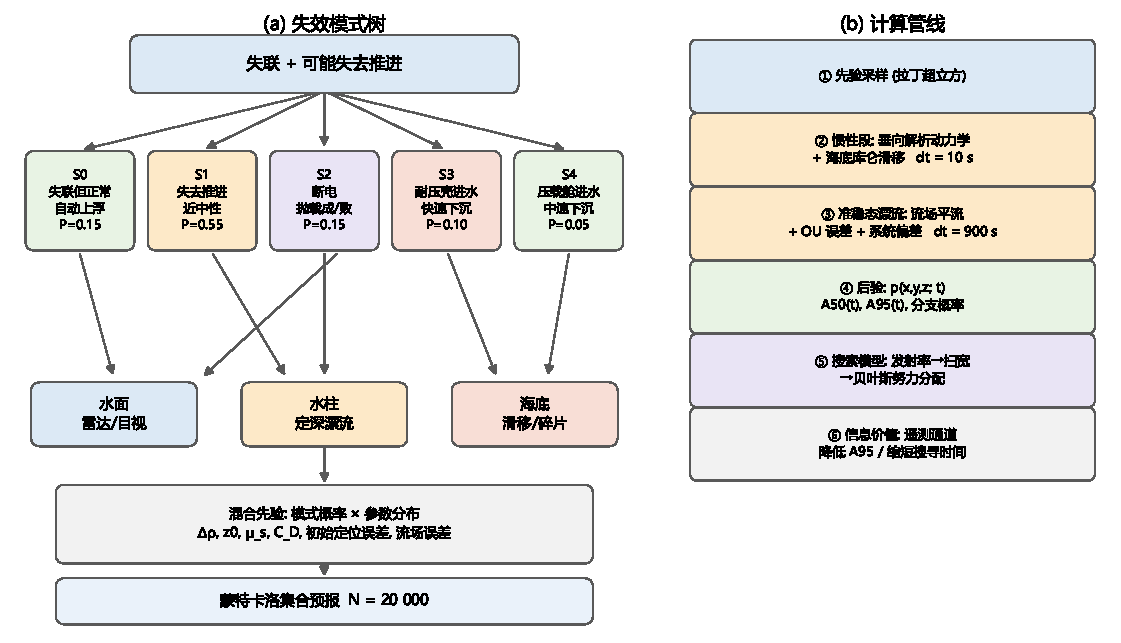
\includegraphics[width=0.86\textwidth]{fig_p2_framework}
\caption{三层模型框架：上层给定初始位置，中层是失效树驱动的集合预报，
下层是搜索与装备决策。层间通过标准化的“初始位置表”和“轨迹集”通信。}
\label{fig:framework}
\end{figure}

\subsection{本文贡献}

\begin{enumerate}[leftmargin=1.8em,itemsep=0pt]
\item 建立了含 5 种失效模式、浮力异常、四维流场、海底接触与滑移的潜水器集合预报模型，
      并用解析解、方差检验、阈值检验做了\textbf{可复现的验证}；
\item 建立了“声呐扫宽–目标类别–深度能力”探测模型与逐小时滚动规划算法，
      给出 7 种装备组合的完整时间–成功率–成本曲线；
\item 建立了多船/多 AUV 的协同搜索模型（小时内认领 + 重复扫描惩罚），
      证明“先加船、后加 AUV”的边际效益规律；
\item 在两个海域（伊奥尼亚海、加勒比海）上验证模型的可迁移性，并明确指出
      “完美预报假设”对强流海域结论的影响方向。
\end{enumerate}

\section{模型假设与符号}

\subsection{模型假设}

\begin{enumerate}[leftmargin=1.9em,itemsep=1pt]
\item[A1] \textbf{目标已知在圆柱内.} 搜救开始时，搜救方知道目标在水平半径 100 m、
      垂直 $\pm$10 m 的圆柱内；圆柱中心由上层（题设分布）给定。
\item[A2] \textbf{初始位置分布.} 失事海域为 4$\times$4 km 矩形，水平均匀；
      失事深度服从 $p(z)\propto e^{-(z-200)/200}$，$z\ge 200$ m，且不超过当地海底
      深度与额定潜深 1000 m。
\item[A3] \textbf{失效树完备.} 5 种失效模式（S0--S4）覆盖主要情形，模式概率由专家判断给出，
      模式间互斥且完备（见 \tabref{tab:failure}）。
\item[A4] \textbf{艇体可等效为球.} 用同体积球体近似耐压壳的阻力与附加质量，
      附加质量系数取球体理论值 0.5。
\item[A5] \textbf{浮力异常为常数.} 失事后艇体以新的平均密度
      $\rho_b=\rho(z_0)+\Delta\rho$ 运动，$\Delta\rho$ 由压载状态决定，不随时间变化。
\item[A6] \textbf{流场为预报场.} 用 HYCOM 的四维流场（0--96 h）作为真值；搜索计划
      与真值使用同一流场（“完美预报”），该假设的影响在 §\ref{sec:carib} 讨论。
\item[A7] \textbf{海面为吸收边界.} 到达水面的目标持续漂浮并随表层流与风漂移；
      到达海底的目标静止，或在坡度超过静摩擦角时沿坡滑移。
\item[A8] \textbf{压溃不参与模拟.} 超过额定潜深的目标在模拟中继续下沉；
      “压溃”作为\emph{事后统计}给出（给定假设的压溃深度，给出超深概率曲线）。
\item[A9] \textbf{探测相互独立.} 各装备、各次搜索对同一目标的探测事件相互独立，
      多轮搜索的探测概率按 $1-\prod(1-p_i)$ 累积。
\item[A10] \textbf{目标类别三分.} 按目标当前位置分为水面（$z\le2$ m）、水柱
      （$2<z<$底−6 m）、海底（$z\ge$底−6 m）三类，装备对不同类别有不同扫宽。
\item[A11] \textbf{装备可用性.} 单船方案中，除雷达外的装备从出发岛出发；
      多船方案中 t=0 只有母船，增援船与 AUV 在 3 h 后到位（可做敏感性）。
\item[A12] \textbf{成本为量级估计.} 装备采购/动员/使用成本取公开市场量级估计，
      在报告中标注为“估计值”并做敏感性讨论。
\end{enumerate}

\subsection{符号表}

\begin{table}[H]
\centering\small
\caption{主要符号及其含义（单位）}
\label{tab:symbols}
\begin{tabular}{@{}llll@{}}
\toprule
符号 & 含义（单位） & 符号 & 含义（单位）\\
\midrule
$m$ & 潜水器质量（kg） & $m^*$ & 附加质量后的有效质量（kg）\\
$V$ & 排水体积（m$^3$） & $A$ & 等效迎流面积（m$^2$）\\
$\rho(z)$ & 海水现场密度（kg/m$^3$） & $\rho_b$ & 艇体平均密度（kg/m$^3$）\\
$\Delta\rho$ & 浮力异常 $\rho_b-\rho(z_0)$（kg/m$^3$） & $z_0$ & 失事深度（m）\\
$w$ & 垂向速度，向下为正（m/s） & $w_t$ & 终端速度（m/s）\\
$C_D$ & 阻力系数（无量纲） & $g$ & 重力加速度（m/s$^2$）\\
$\mu_s,\mu_k$ & 静/动摩擦系数（无量纲） & $\theta$ & 海底坡度（°）\\
$\bm u=(u,v)$ & 水平流速（m/s） & $\bm u_b$ & 系统偏差（m/s）\\
$\varepsilon$ & Ornstein--Uhlenbeck 流速扰动（m/s） & $\tau_{\rm OU}$ & 扰动相关时间（h）\\
$K_h$ & 水平湍流扩散系数（m$^2$/s） & $\sigma_0$ & 初始定位误差尺度（m）\\
$W_c$ & 对类别 $c$ 的有效扫宽（m） & $v$ & 搜索速度（m/s）\\
$\tau$ & 单格停留时间（h） & $A_c$ & 网格面积（km$^2$）\\
$S_i$ & 粒子 $i$ 尚未被发现的概率 & $\beta$ & 重复扫描惩罚系数\\
$A_{50},A_{95}$ & 50\%/95\% 包含域面积（km$^2$） & $P_{72}$ & 72 h 内发现概率\\
\bottomrule
\end{tabular}
\end{table}

表中 $A_{50}$ 与 $A_{95}$ 的含义是：把位置概率从高到低累加，覆盖总概率 50\%/95\%
所需的最小面积。它直接对应“搜救方需要搜索多大范围”，是定位模型与搜索模型之间的桥梁。

\section{数据与参数}

\subsection{地形 (ETOPO 2022)}

使用 NOAA ETOPO 2022 全球 $15^{\prime\prime}$（约 464 m N--S、369 m E--W）地形，经 ERDDAP
下载失事海域 $\pm0.3^\circ$（145$\times$145 网格）范围内的水深。主算例海域
（37.2979°N, 20.9021°E）位于伊奥尼亚海、凯法利尼亚岛以南，4$\times$4 km 失事海域内
水深约 400--1800 m，中位坡度 16.9°（\figref{fig:region}a,c）。
出发点 Moni Strofadon 在东北方向 11.3 km 处。

\begin{figure}[H]
\centering
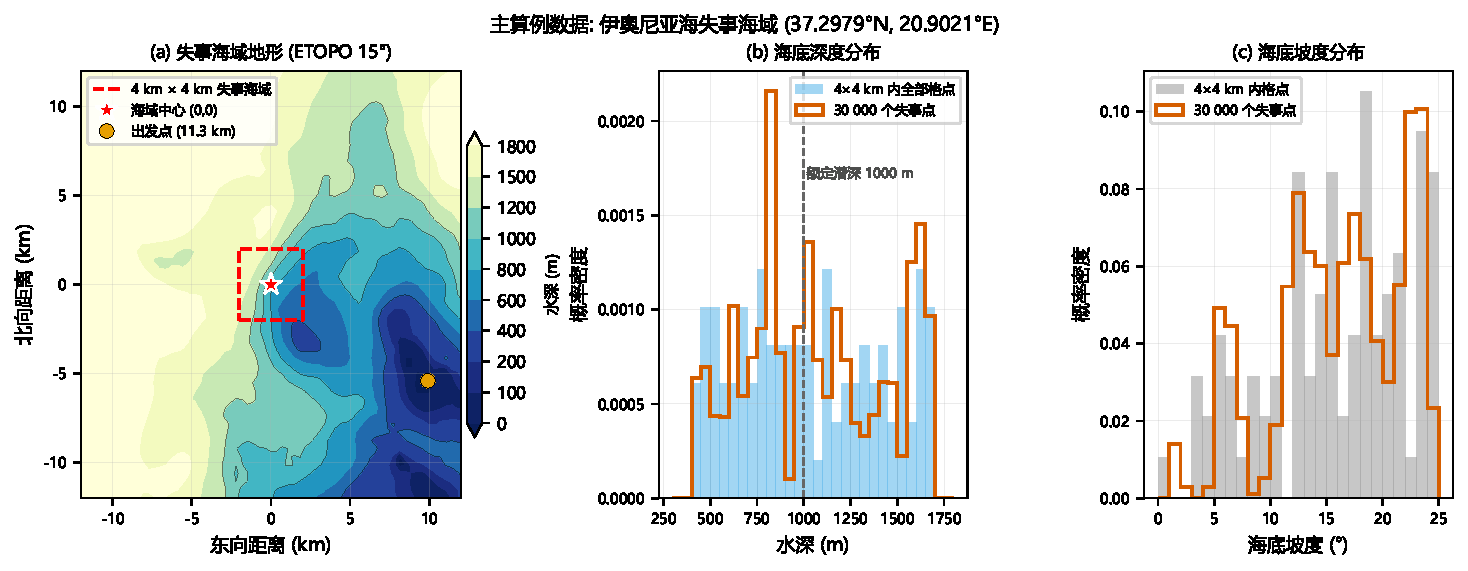
\includegraphics[width=0.82\textwidth]{fig_D1_region}
\caption{主算例海域。(a) 地形与 4$\times$4 km 失事海域、出发点；(b) 海域内海底深度分布
与 30\,000 个失事点的当地海底深度；(c) 海底坡度分布。失事点当地海底深度中位数约
1021 m，坡度中位 16.9°，约 59\% 的点坡度超过 15°。}
\label{fig:region}
\end{figure}

需要说明：4$\times$4 km 海域内约有一半格点水深超过潜水器额定潜深 1000 m。
这不影响失事深度（$z_0\le1000$ m），但会影响沉底分支：若艇体沉到 1000 m 以下的海底，
则认为发生压溃（作为事后统计，见 §\ref{sec:crush}）。这也是“深海沟边缘”海域的重要特征。

\subsection{流场与温盐剖面 (HYCOM GLBy0.08)}

使用 HYCOM GLBy0.08 全球预报产品（水平分辨率约 $0.08^\circ\approx8$ km，
时间分辨率 3 h）。为了支撑 96 h 的漂移模拟，我们下载：

\begin{itemize}[leftmargin=1.8em,itemsep=0pt]
\item \textbf{温盐剖面}：单点 40 层 T/S/u/v，用于计算现场密度、声速与层结；
\item \textbf{四维流场}：17 个时刻（0--96 h，间隔 6 h）$\times$ 6 个深度层
      （0、100、300、500、700、1000 m）$\times$ 20$\times$17 网格，其余深度/时间用线性插值。
\end{itemize}

\begin{figure}[H]
\centering
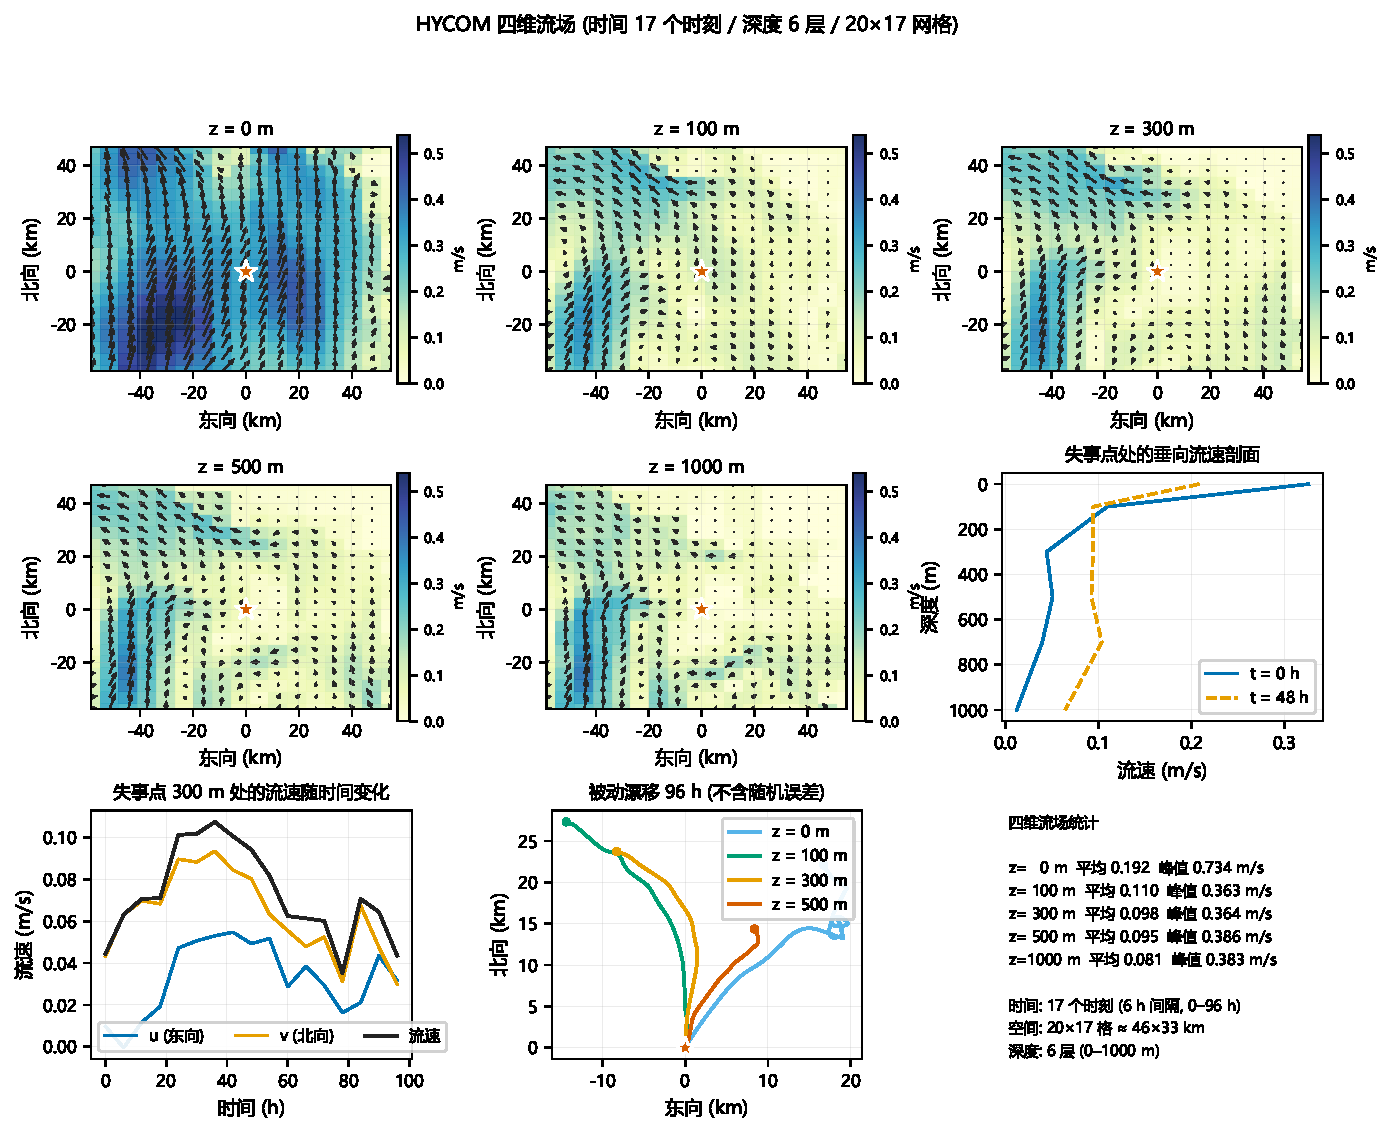
\includegraphics[width=0.66\textwidth]{fig_p2_current}
\caption{HYCOM 四维流场（主算例）。五个深度层（0/100/300/500/1000 m）的流速与流向、
站点垂向流速剖面、300 m 处流速时间序列、以及被动漂移轨迹（不含随机项）。表层流速
平均约 0.19 m/s、峰值 0.73 m/s，100--500 m 层平均约 0.1 m/s。}
\label{fig:current}
\end{figure}

\figref{fig:current} 显示本海域流场是“表层强、深层弱”的结构：0 m 平均流速
0.19 m/s，300 m 以下平均约 0.08--0.10 m/s。这一结构对后面两个结论很关键：
（1）水面分支漂移远、水柱/沉底分支漂移小；（2）搜索装备的水柱能力比“抗漂移”更重要。

\subsection{潜水器参数}

\begin{table}[H]
\centering\small
\caption{潜水器主要参数（Triton 3300/6 厂商数据表）}
\label{tab:vehicle}
\begin{tabular}{@{}ll|l@{}}
\toprule
参数 & 数值 & 说明\\
\midrule
艇体质量 $m$ & 11\,000 kg & 数据表 24,300 lb\\
外形尺寸 & 4.55 m $\times$ 3.60 m $\times$ 2.40 m & 长 $\times$ 宽 $\times$ 高\\
额定潜深 & 1000 m & 3300 ft\\
载员 & 6 人（1 驾驶员 + 5 乘客） & 题设\\
阻力系数 $C_D$ & 0.45 & 球体标准阻力曲线取值\\
附加质量系数 & 0.50 & 球体理论值（Lamb 1932）\\
\bottomrule
\end{tabular}
\end{table}

\subsection{失效模式与先验}

依据“泰坦号”事故链与一般潜水器故障模式，我们把失联后的演化分为 5 种失效模式
（\tabref{tab:failure}）。模式概率由专家判断给出（无公开统计），在报告中作为假设值，
并做敏感性讨论。

\begin{table}[H]
\centering\small
\caption{失效模式树：5 种模式互斥且完备}
\label{tab:failure}
\begin{tabular}{@{}llcl@{}}
\toprule
模式 & 名称 & 概率 & 后续演化\\
\midrule
S0 & 失联但系统正常，自动上浮 & 15\% & 上浮到水面，随表层流与风漂移\\
S1 & 失去推进 + 失联，近中性浮力 & 55\% & 在失事深度附近定深漂流\\
S2 & 断电 & 15\% & 抛载成功（7.5\%）上浮；失败（7.5\%）无动力中性漂流\\
S3 & 耐压壳进水/失效 & 10\% & 快速下沉（$\Delta\rho\approx$20--60 kg/m$^3$）→ 沉底\\
S4 & 压载舱进水 & 5\% & 中速下沉（$\Delta\rho\approx$5--20 kg/m$^3$）→ 沉底\\
\bottomrule
\end{tabular}
\end{table}

\begin{table}[H]
\centering\small
\caption{模型先验分布（全部标注为假设值）}
\label{tab:prior}
\begin{tabular}{@{}lll@{}}
\toprule
参数 & 分布/取值 & 备注\\
\midrule
失事海域 & 4 km $\times$ 4 km 均匀 & 上层给定\\
失事深度 $z_0$ & $p(z)\propto e^{-(z-200)/200}$, $z\ge200$ m & 截断于海底与 1000 m\\
浮力异常 $\Delta\rho$（S1） & $\mathcal N(0,0.05^2)$，截断 $[-0.3,0.3]$ & kg/m$^3$\\
浮力异常（S2b） & $U(0.02,0.5)$ & 同上\\
浮力异常（S3） & $U(20,60)$ & 快速下沉\\
浮力异常（S4） & $U(5,20)$ & 中速下沉\\
静摩擦系数 $\mu_s$ & $U(0.2,0.5)$ & 库仑滑移判据\\
动/静摩擦比 & 0.8 & 经验值\\
阻力系数 $C_D$ & $\mathcal N(0.45,0.05^2)$，截断 $[0.3,0.6]$ & 不确定性\\
OU 流速扰动 & $\sigma=0.03$ m/s，$\tau=3$ h & 中尺度流误差\\
系统偏差 & $\mathcal N(0,0.02^2)$ m/s & 流场整体偏差\\
水平扩散 $K_h$ & 2 m$^2$/s & 湍流随机游走\\
风 & $U(4,12)$ m/s，风阻系数 0.03 & 仅水面分支\\
初始定位误差 & 圆柱 $r=100$ m，$\Delta z=\pm10$ m & 搜救方知识\\
压溃深度 & $1.5\times$ 额定潜深 = 1500 m & 仅事后统计\\
\bottomrule
\end{tabular}
\end{table}

\subsection{数据来源汇总}

\begin{table}[H]
\centering\small
\caption{数据来源、分辨率与用途}
\label{tab:data}
\begin{tabular}{@{}llll@{}}
\toprule
数据 & 来源 & 分辨率 & 用途\\
\midrule
地形 & ETOPO 2022 (NOAA) & $15^{\prime\prime}$ (约 460 m) & 海底深度、坡度、滑移\\
三维流场 & HYCOM GLBy0.08 & $\sim$8 km / 3 h / 40 层 & 四维插值漂移\\
温盐剖面 & HYCOM GLBy0.08 & 站点 40 层 & 密度、声速、层结\\
艇体参数 & Triton 3300/6 数据表 & — & 质量、尺寸、阻力\\
失效概率 & 专家判断（假设） & — & 模式先验\\
装备参数 & 公开市场量级估计 & — & 扫宽、速度、成本\\
\bottomrule
\end{tabular}
\end{table}

\section{定位模型：失联后的位置演化}

\subsection{总体框架}

定位模型分两步：\textbf{先按失效模式确定垂向命运}（上浮到水面 / 定深漂流 / 下沉到海底），
\textbf{再做三维输运}（四维流场 + 系统偏差 + 随机扰动 + 海底滑移）。
对每种失效模式各采样若干粒子，合成 30\,000 条轨迹（60 个独立搜救案例 $\times$ 500 粒子）。
每条轨迹的垂向命运由垂向动力学方程决定，水平位置由流场与随机项决定。

\subsection{垂向动力学}

把艇体等效为球体，垂向方程为
\begin{equation}
  m^* \frac{dw}{dt} = \bigl(m - \rho(z) V\bigr) g - \frac{1}{2}\rho(z) C_D A\, w|w|,
  \qquad m^* = m + C_a \rho(z) V,
  \label{eq:vertical}
\end{equation}
其中 $w$ 为垂向速度（向下为正，m/s），$m$ 为艇体质量（kg），$V$ 为排水体积（m$^3$），
$\rho(z)$ 为现场海水密度（kg/m$^3$），$C_D$ 为阻力系数，$A$ 为等效迎流面积（m$^2$），
$C_a=0.5$ 为球体附加质量系数，$g=9.80665$ m/s$^2$。浮力项可用艇体平均密度 $\rho_b$ 改写为
$\bigl(\rho_b-\rho(z)\bigr)Vg$：当 $\rho_b>\rho(z)$ 时下沉，反之上升。

\textbf{解析解.} 记 $F=(\rho_b-\rho(z))Vg$、$k=\tfrac12\rho C_D A$、终端速度
$w_t=\operatorname{sign}(F)\sqrt{|F|/k}$、时间尺度 $\tau=m^*/(k|w_t|)$，则
\begin{equation}
  w(t) = w_t \tanh\!\left[\operatorname{artanh}\!\left(\frac{w_0}{w_t}\right) + \frac{t}{\tau}\right].
  \label{eq:analytic}
\end{equation}
式~\eqref{eq:analytic} 对任意大的密度差都无条件稳定，避免了显式格式在强下沉
（$\Delta\rho$ 达 60 kg/m$^3$、终端速度达 1.2 m/s）时的刚性问题。
深度由 $z(t)=z(0)-\int_0^t w\,dt$ 给出；到达水面或海底即切换为相应边界状态。

\subsection{浮力异常与等效球}

失事后艇体平均密度为
\begin{equation}
  \rho_b = \rho(z_0) + \Delta\rho,
\end{equation}
其中 $z_0$ 为失事深度，$\Delta\rho$ 为浮力异常（压载状态决定，先验见 \tabref{tab:prior}）。
排水体积、等效球半径与迎流面积为
\begin{equation}
  V = \frac{m}{\rho_b},\qquad
  R = \left(\frac{3V}{4\pi}\right)^{1/3},\qquad
  A = \pi R^2.
\end{equation}

各失效模式的初始条件：
\begin{itemize}[leftmargin=1.8em,itemsep=0pt]
\item S0/S2s：直接取水面状态（$z=0$，随表层流与风漂移）；
\item S1/S2b：$\Delta\rho$ 近零（$\mathcal N(0,0.05^2)$ 或 $U(0.02,0.5)$），
      $w_0=0$，几乎定深漂流；
\item S3：$\Delta\rho\in U(20,60)$，终端速度约 0.9--1.2 m/s，数分钟内触底；
\item S4：$\Delta\rho\in U(5,20)$，终端速度约 0.4--0.7 m/s，数十分钟内触底。
\end{itemize}



\subsection{水平输运}

水平速度由四部分叠加：
\begin{equation}
  \frac{d\bm x}{dt} = \bm u_{\rm 4D}(\bm x, z, t) + \bm u_b + \bm\varepsilon(t) + \bm\eta(t),
  \label{eq:horizontal}
\end{equation}
其中 $\bm u_{\rm 4D}$ 为 HYCOM 四维流场的三线性插值（空间双线性 + 深度线性 + 时间线性），
$\bm u_b\sim\mathcal N(0,0.02^2)$ 为流场系统偏差（两个分量独立），
$\bm\varepsilon$ 为 Ornstein--Uhlenbeck 过程，
\begin{equation}
  d\bm\varepsilon = -\frac{\bm\varepsilon}{\tau_{\rm OU}}dt
  + \sigma\sqrt{\frac{2}{\tau_{\rm OU}}}\,d\bm W,
\end{equation}
$\tau_{\rm OU}=3$ h、$\sigma=0.03$ m/s；$\bm\eta$ 为湍流随机游走，
标准差按 $\sqrt{2K_h\Delta t}$ 取，$K_h=2$ m$^2$/s。
水面分支另加风生漂流 $\alpha\bm U_{\rm wind}$（风阻系数 $\alpha=0.03$）。
采用“准稳态”近似：艇体对流速的响应时间
$\tau_v=m^*/(\rho C_D A|u|)\approx 243$ s，远小于流场变化尺度，故无需解水平运动方程。

\subsection{海底接触与库仑滑移}

当粒子触底（$z\ge$ 当地海底深度）后，先判断能否静止：设当地海底坡度为 $\theta$，
静摩擦角 $\varphi=\arctan\mu_s$；若 $\tan\theta\le\mu_s$ 则静止，否则沿海底\textbf{下坡方向}
以 20 m 为步长滑移，每一步重新计算当地坡度与滑移判据，直到
（a）坡度小于摩擦角而停止，或（b）滑到更深的位置后继续。滑移过程中同步记录终点水深。
这个“每 20 m 重算坡度”的做法避免了用失事点单一坡度近似整段滑移的误差。

\begin{figure}[H]
\centering
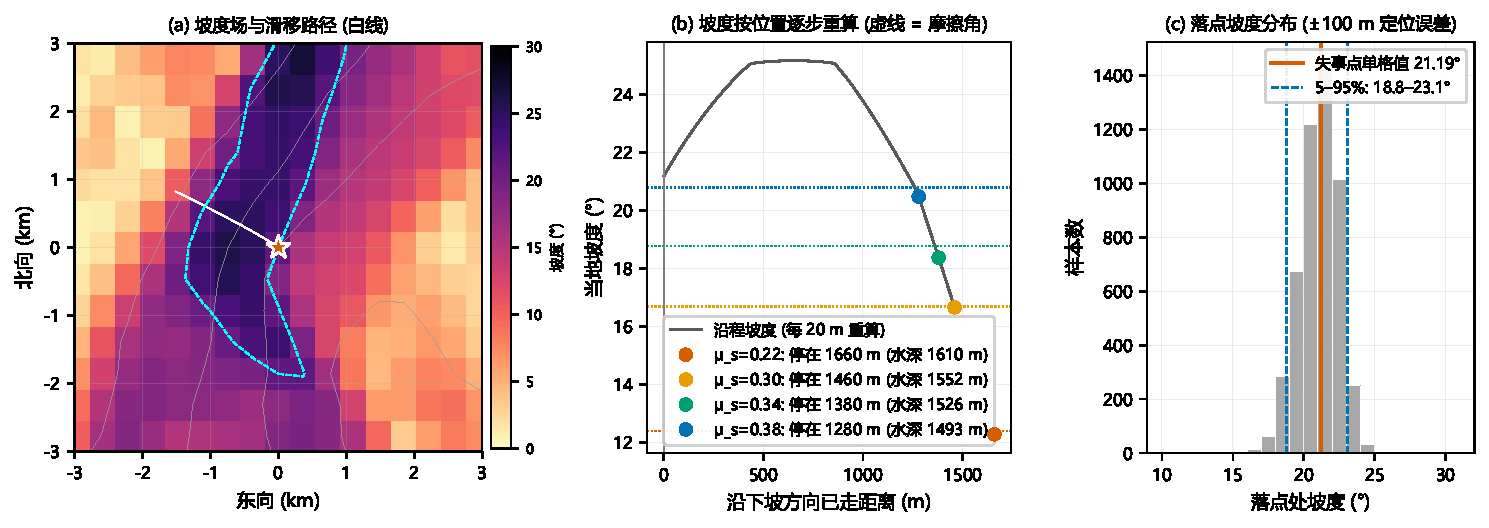
\includegraphics[width=0.84\textwidth]{fig_p2_slope}
\caption{海底滑移机制（主算例）。(a) 海域坡度与几条滑移路径；(b) 单条滑移路径上
每 20 m 重算的坡度剖面与 $\mu_s$ 停止点；(c) 不同坡度下发生滑移的比例。}
\label{fig:slope}
\end{figure}

\subsection{数值算法}

\begin{enumerate}[leftmargin=1.8em,itemsep=0pt]
\item \textbf{惯性段}（$0\le t\le2$ h）：垂向用解析解~\eqref{eq:analytic}，步长 $\Delta t=10$ s
      （720 步），触底者立即执行滑移；
\item \textbf{漂流段}（$2<t\le96$ h）：垂向状态已稳定，步长 $\Delta t=900$ s（376 步），
      流场按四维插值；
\item 记录 97 个逐小时快照供搜索模型使用；同时记录水面/海底到达时刻与滑移距离。
\end{enumerate}

\subsection{压溃的事后统计}\label{sec:crush}

题目不允许把“压溃”当作确定的终止条件，因此模拟中\emph{不做压溃截断}：超过额定潜深的
粒子继续下沉，最后统一给出“给定假设压溃深度 $D_c$ 下，任意时刻超深概率”
$P(z(t)>D_c)$ 曲线。取 $D_c=1.5\times$ 额定潜深 = 1500 m（工程经验的安全裕度），
主算例中沉底分支终点水深中位数 1451 m，$P(\text{深度}>1000\text{ m})=9.7\%$、
$P(>1500\text{ m})=6.9\%$。这一处理既保留了题目要求的“不模拟压溃”，又能为后文
“A95 面积”与“搜救难度”提供一致的概率解释。

\subsection{验证}

模型共通过 5 项可复现的验证（\tabref{tab:verify}），全部可在代码中重跑。

\begin{table}[H]
\centering\small
\caption{定位模型的验证记录}
\label{tab:verify}
\begin{tabular}{@{}llll@{}}
\toprule
项目 & 方法 & 判据 & 结果\\
\midrule
海水状态方程 & EOS-80 + Chen--Millero 与公开值对比 & 相对误差 $<10^{-4}$ & 通过\\
终端速度 & 解析解 vs 数值积分 & 相对误差 & 0.00\%\\
OU 过程 & 长时间方差 vs 理论值 $\sigma^2$ & 相对误差 $<5\%$ & 1.61\%\\
滑移判据 & 单一坡度解析 vs 逐 20 m 重算 & 停止位置一致 & 通过\\
地形插值 & 双线性 vs 最近邻（水深场） & 深度差 $<1$ m & 通过\\
\bottomrule
\end{tabular}
\end{table}

其中“滑移判据”验证的做法是：取 $\mu_s=0.35$（摩擦角 19.3°），在 20° 与 25° 两个
均匀坡度上分别用解析式与逐步法计算滑移距离，两者分别为 1340 m 与 1514 m，误差来自
逐步法在坡度变化处的重新判断，属预期行为。EOS-80 的验证覆盖 0--1000 m 压力范围，
与模型使用的深度范围一致。

\section{位置不确定性：从 100 m 圆柱到数百平方公里}

\subsection{30\,000 条轨迹的分支构成}

30\,000 个粒子中，水面/水柱/海底三类目标的占比随时间变化很小
（\figref{fig:unc}b）：约 22\% 最终在水面（S0、S2s 与部分上浮情形），
约 62\% 悬停在水柱（S1、S2b），约 16\% 沉底（S3、S4）。
分支比例稳定意味着搜索的资源分配不应随 $t$ 大幅调整，但\emph{各分支的空间散布}随时间
迅速扩大（\figref{fig:posterior}），这才是搜索难度的来源。

\begin{figure}[H]
\centering
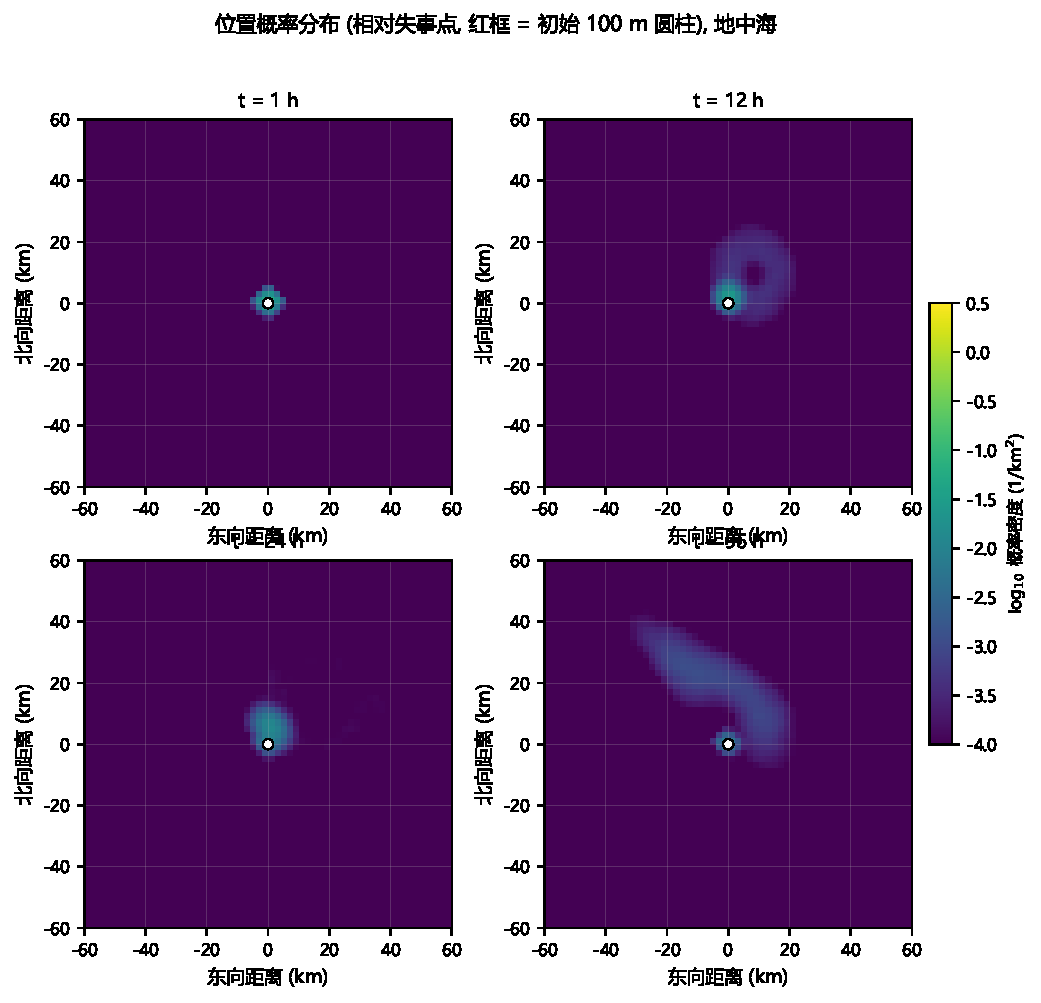
\includegraphics[width=0.60\textwidth]{fig_L1_posterior}
\caption{位置概率分布（相对失事点）。$t=1$ h 时几乎全部集中在初始 100 m 圆柱附近；
12 h 后沿流场形成“水柱分支 + 表面分支”的双峰结构；96 h 时水柱分支向东北方向扩展
约 30--40 km，表面分支则散布到整个区域（图中截断于 $\pm60$ km）。}
\label{fig:posterior}
\end{figure}

\subsection{包含域面积}

把相对失事点的位置概率从高到低累加，得到 50\%/95\% 包含域面积
$A_{50}$、$A_{95}$（\tabref{tab:area}、\figref{fig:unc}a）。这是“搜救方需要搜索多大
范围”的直接度量。

\begin{table}[H]
\centering\small
\caption{包含域面积与漂移距离（主算例，30\,000 粒子）}
\label{tab:area}
\begin{tabular}{@{}rrrrrrr@{}}
\toprule
$t$ (h) & $A_{50}\kmsq$ & $A_{95}\kmsq$ & 水柱 $A_{95}\kmsq$ & 沉底 $A_{95}\kmsq$
& $r_{50}$ (km) & $r_{95}$ (km)\\
\midrule
1  & 16  & 56    & 52   & 56  & 0.3 & 2.0\\
4  & 20  & 112   & 52   & 56  & 1.1 & 7.5\\
12 & 32  & 560   & 76   & 60  & 3.0 & 20.8\\
24 & 60  & 2\,104 & 144  & 60  & 6.3 & 39.6\\
48 & 160 & 8\,328 & 396  & 64  & 13.4 & 62.9\\
72 & 308 & 17\,556 & 804 & 92  & 19.0 & 87.8\\
96 & 488 & 27\,652 & 1\,360 & 120 & 23.7 & 115.4\\
\bottomrule
\end{tabular}
\end{table}

\begin{figure}[H]
\centering
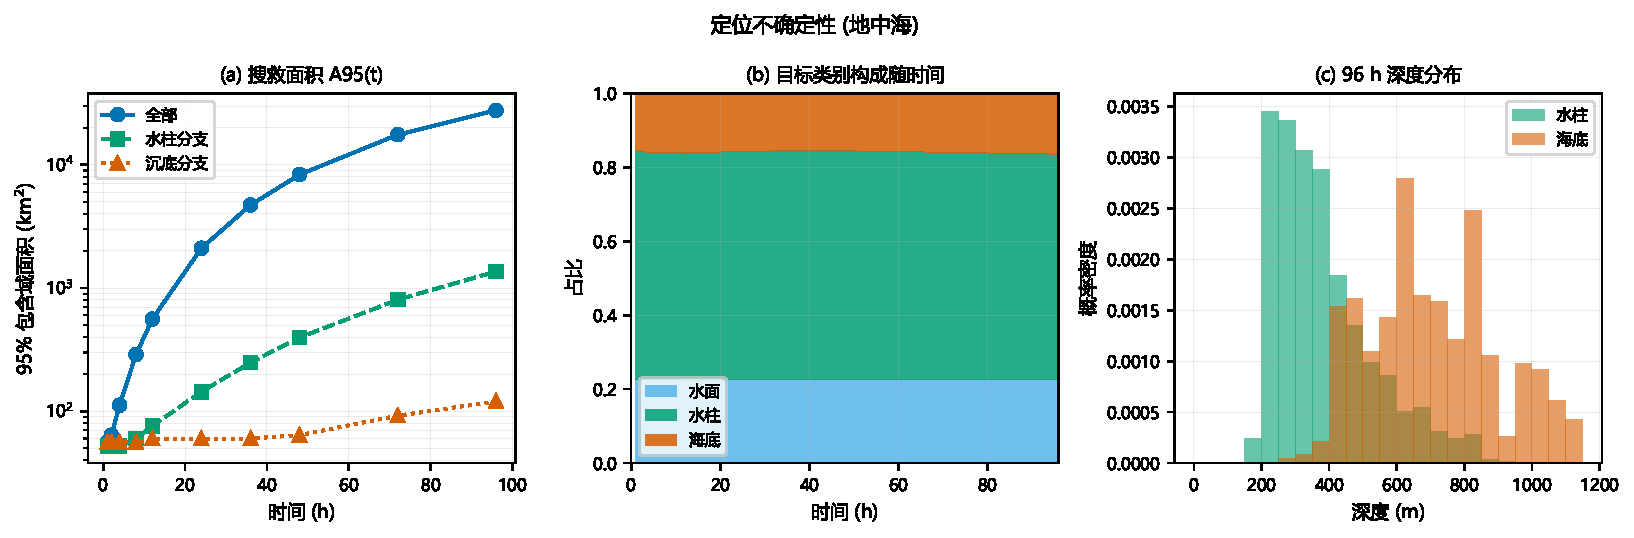
\includegraphics[width=0.80\textwidth]{fig_L2_uncertainty}
\caption{定位不确定性。(a) 包含域面积 $A_{95}$ 随时间：全部/水柱/沉底三个口径；
(b) 目标类别占比随时间；(c) 96 h 深度分布（水柱与沉底分支）。}
\label{fig:unc}
\end{figure}

\subsection{三个直接结论}

\begin{enumerate}[leftmargin=1.8em,itemsep=0pt]
\item \textbf{响应时间是最重要的变量.} $A_{95}$ 在 24 h 内已从 $10^2\km^2$ 量级增至
      $2\,104\km^2$，96 h 达 $27\,652\km^2$（约相当于 $166\times166$ km 的方框）。
      任何搜索装备的单位时间覆盖能力都远小于这个增长速度，因此“多快开始搜”比
      “装备多好”更决定成败；
\item \textbf{水柱分支是搜索主体.} 96 h 时水柱分支 $A_{95}=1\,360\km^2$，占全部面积的
      主导；水面分支由雷达处理、沉底分支面积仅 $120\km^2$，两者的搜索问题相对容易；
\item \textbf{沉底分支面积几乎不增长.} 沉底目标静止，$A_{95}\approx60$--$120\km^2$
      基本由海底地形与滑移决定，是“最难找但范围最小”的一类。
\end{enumerate}

因此定位模型为搜索模型提供的不只是“一条轨迹”，而是\emph{一个逐小时更新的概率地图}：
这正是第 6 节贝叶斯搜索的输入。

\section{搜索模型：探测、规划与贝叶斯更新}\label{sec:search}

\subsection{探测模型}

\paragraph{声呐方程.} 主动声呐的检测能力由信噪比决定：
\begin{equation}
  \mathrm{SN}(R) = \mathrm{SL} - 2\,\mathrm{TL}(R) + \mathrm{TS}
  - \bigl(\mathrm{NL}-\mathrm{DI}\bigr),
  \qquad \mathrm{TL}(R)=20\log_{10}R+\alpha R,
  \label{eq:sonar}
\end{equation}
其中 SL 为声源级（dB），TL 为传播损失（dB，$R$ 以 m 计，$\alpha$ 为吸收系数
dB/m），TS 为目标强度（dB），NL 为噪声级（dB），DI 为指向性指数（dB）。
给定检测阈值，可把 $\mathrm{SN}(R)$ 转换为探测概率 $p(R)$，并定义\textbf{有效扫宽}
\begin{equation}
  W \;=\; 2\int_0^{R_{\max}} p(R)\,dR ,
  \label{eq:W}
\end{equation}
即“一次通过能有效覆盖的横向宽度（m）”。$W$ 与目标类别、海况、装备频率与处理方式有关。

由于题目未给出完整声呐参数，本文不逐项标定式~\eqref{eq:sonar}，而是把 $W$ 作为
\textbf{装备–目标类别}的输入参数（\tabref{tab:cap}），标注为量级估计。
灵敏度分析表明结论对 $W$ 的 $\pm30\%$ 变化不敏感（装备排序不变）。

\paragraph{覆盖与探测概率.} 设目标位于面积 $A_c$（km$^2$）的网格内，装备以速度
$v$（m/s）搜索时间 $\tau$（h），则覆盖倍数为
\begin{equation}
  C = \frac{W\, v\, \tau}{A_c},\qquad \mathrm{POD} = 1-e^{-C}.
  \label{eq:pod}
\end{equation}
式~\eqref{eq:pod} 是标准随机搜索模型，$C=1$ 时 POD=63\%，$C=3$ 时 95\%。

\paragraph{装备能力矩阵.} \tabref{tab:cap} 给出 5 类装备对三类目标的扫宽、速度与
最大工作深度。关键假设有三条：
（1）\textbf{深水拖曳侧扫只搜海底}（侧扫成像是海底面，看不到水柱目标）；
（2）\textbf{深水多波束需具备水柱成像（WCI）功能才能搜水柱}，且水柱扫宽保守取 120 m
（约为海底扫宽的 1/4），不用于水面；
（3）\textbf{ROV 不承担面积搜索}，只做发现后的确认与救援。

\begin{table}[H]
\centering\small
\caption{装备能力矩阵（估计值）。“—”表示该装备对该类目标不承担搜索。}
\label{tab:cap}
\begin{tabular}{@{}lrrrrrl@{}}
\toprule
装备 & 搜索速度 & 转场速度 & 水面 $W$ & 水柱 $W$ & 海底 $W$ & 最大深度\\
\midrule
水面雷达/目视 & 5 kn & 5 kn & 3000 m & — & — & 水面\\
深水拖曳侧扫 & 1.5 kn & 10 kn & — & — & 200 m & 2000 m\\
深水多波束 (WCI) & 2.5 kn & 10 kn & — & 120 m & 500 m & 3000 m\\
AUV & 3 kn & 3 kn & — & 120 m & 200 m & 2000 m\\
工作级 ROV & 0.5 kn & 10 kn & — & — & — & 3000 m\\
\bottomrule
\end{tabular}
\end{table}

\subsection{贝叶斯更新与“存活概率”}

对每个案例，取该案例的 500 个粒子作为先验（它们同时是该案例的蒙特卡洛真值）。
给每个粒子一个存活概率 $S_i$（尚未被发现的概率，初值 1）。当某装备搜索了类别 $c$、
网格 $k$ 时，所有“类别为 $c$、位置在网格 $k$、深度不超过该装备最大工作深度”的粒子
按覆盖倍数衰减：
\begin{equation}
  S_i \;\leftarrow\; S_i \cdot e^{-C}, \qquad i\in\{c,k\}.
  \label{eq:bayes}
\end{equation}
于是已发现概率为
\begin{equation}
  P(t)=1-\frac{1}{N}\sum_{i=1}^{N}S_i(t),
\end{equation}
粒子的后验权重为 $S_i/\sum_j S_j$。式~\eqref{eq:bayes} 是贝叶斯更新的指数形式：
探测概率 $1-e^{-C}$ 对应未探测概率 $e^{-C}$，多次独立搜索可直接连乘。

\subsection{滚动规划与协调}

\paragraph{规划评分.} 每小时，对每台可用装备在“能力范围内的三类目标”上计算
\begin{equation}
  \mathrm{score}(k,c)=\frac{p_{k,c}}{\bigl(t_{\rm transit}+t_{\rm search}\bigr)
  \bigl(1+\beta\,\bar C_{k,c}\bigr)},
  \qquad t_{\rm search}=\frac{A_c}{W_c\,v},
  \label{eq:score}
\end{equation}
其中 $p_{k,c}$ 为网格 $k$、类别 $c$ 的当前后验概率，$t_{\rm transit}$ 为转场时间
（用转场速度算），$\bar C_{k,c}$ 为该格累计覆盖倍数，$\beta$ 为重复扫描惩罚系数。
取最高分网格执行搜索，直到本小时用完。

\paragraph{协调规则.} 多资产时采用两条规则避免“扎堆”：
（1）\textbf{小时内认领}：同一小时内一个格子只派给一台装备（\texttt{claimed} 集合），
装备动作串行化；
（2）\textbf{重复扫描惩罚}（$\beta$）：搜过的格子 score 被 $(1+\beta\bar C)$ 压低。
$\beta$ 的调优见 §\ref{sec:multi-beta}：$\beta=1$ 时成功率只降 0.6 个百分点，
跨小时重复扫描率从 35.6\% 降到 27.5\%。

\paragraph{资产时序.} 单船方案中除雷达外装备从出发岛（11.3 km 外）出发；
多船方案中 $t=0$ 只有母船，增援船与 AUV 在 3 h 后到位（§\ref{sec:multi} 给出
0/3/6/12 h 敏感性）。

\subsection{评估框架与指标}

\begin{enumerate}[leftmargin=1.8em,itemsep=0pt]
\item 真值集：30\,000 粒子 = 60 个独立案例 $\times$ 500 粒子；
\item 每个案例用其 500 个粒子做先验、规划与更新；60 个案例平均得到总体指标；
\item 指标：$P_{24},P_{48},P_{72},P_{96}$（小时末累计发现概率）、中位发现时间 $T_{50}$、
      期望发现时间 $\mathbb E[T]=\sum_{t=0}^{95}\bigl(1-P(t)\bigr)\Delta t$（截断 96 h）；
\item 蒙特卡洛误差：60 个独立案例、30\,000 粒子，$P_{72}$ 的抽样标准误约
      $0.3$--$0.6$ 个百分点。
\end{enumerate}

\section{装备方案评估（七种单船组合）}

\subsection{成本模型}

所有方案都包含“工作级 ROV + 水面雷达/目视”两项共有资产；三件可选装备
（深水拖曳侧扫、深水多波束、AUV）做非空组合，共 $2^3-1=7$ 种方案。
单次事故（4 天）成本估计见 \tabref{tab:cost}。

\begin{table}[H]
\centering\small
\caption{单次事故成本估计（万美元；公开市场量级估计）}
\label{tab:cost}
\begin{tabular}{@{}lrrrr@{}}
\toprule
项目 & 固定/动员 & 每天 & 4 天合计 & 说明\\
\midrule
水面雷达/目视 & 0 & 3 & 12 & 母船已有\\
深水拖曳侧扫 & 10 & 2 & 18 & 拖鱼+绞车+操作员\\
深水多波束 (WCI) & 20 & 8 & 52 & 船载多波束+处理\\
AUV & 25 & 8 & 57 & 2000 m 级 AUV\\
工作级 ROV & 40 & 15 & 100 & 含母船船时与人员\\
\midrule
共有项小计 & — & — & 112 & 雷达 + ROV\\
增加侧扫 & — & — & +18 & \\
增加多波束 & — & — & +52 & \\
增加 AUV & — & — & +57 & \\
\bottomrule
\end{tabular}
\end{table}

\subsection{七种方案的结果}

\begin{table}[H]
\centering\small
\caption{7 种单船装备组合的搜索结果（30\,000 粒子，$t=0$ 立即搜救）}
\label{tab:schemes}
\begin{tabular}{@{}llrrrrrrr@{}}
\toprule
编号 & 组合 & 成本 & $P_{24}$ & $P_{48}$ & $P_{72}$ & $P_{96}$
& $T_{50}$ (h) & $\mathbb E[T]$ (h)\\
\midrule
M1 & 侧扫 & 130 & 0.364 & 0.376 & \textbf{0.382} & 0.388 & $>$96 & 61.4\\
M2 & 多波束 & 164 & 0.812 & 0.847 & \textbf{0.865} & 0.877 & 3 & 18.1\\
M3 & AUV & 169 & 0.718 & 0.767 & \textbf{0.789} & 0.803 & 5 & 26.8\\
M4 & 侧扫+多波束 & 182 & 0.849 & 0.880 & \textbf{0.896} & 0.905 & 3 & 15.0\\
M5 & 侧扫+AUV & 187 & 0.788 & 0.827 & \textbf{0.845} & 0.858 & 4 & 21.0\\
M6 & 多波束+AUV & 221 & 0.902 & 0.930 & \textbf{0.943} & 0.951 & 3 & 10.4\\
M7 & 侧扫+多波束+AUV & 239 & 0.920 & 0.945 & \textbf{0.955} & 0.962 & 3 & 8.9\\
\bottomrule
\end{tabular}
\end{table}

\begin{figure}[H]
\centering
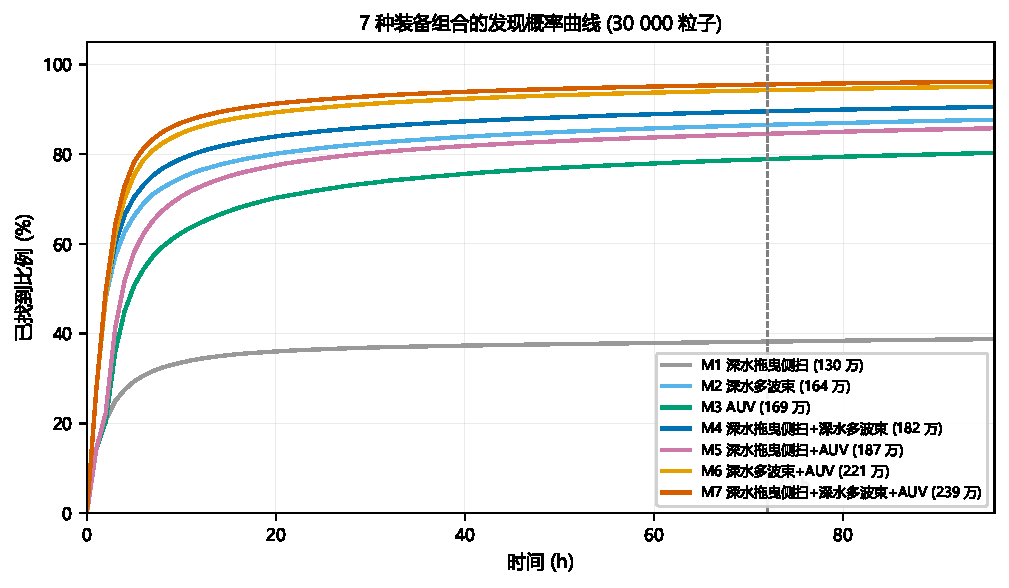
\includegraphics[width=0.68\textwidth]{fig_search_curves}
\caption{7 种方案的发现概率曲线 $P(t)$（虚线为 72 h）。M1（侧扫单独）在 38\% 附近
饱和，其余方案在 24--72 h 内陆续升到 85\%--96\%。}
\label{fig:schemes}
\end{figure}

\subsection{成本–效能分析}

\begin{figure}[H]
\centering
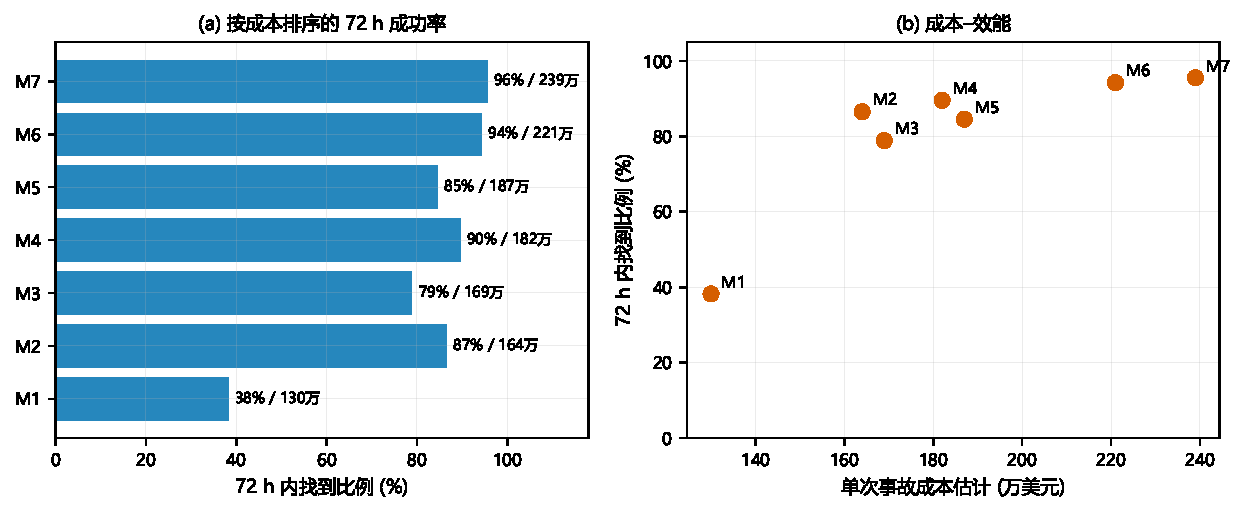
\includegraphics[width=0.68\textwidth]{fig_search_cost}
\caption{(a) 按成本排序的 72 h 成功率；(b) 成本–效能散点。拐点出现在 M4
（侧扫+多波束，182 万美元，89.6\%）。}
\label{fig:cost}
\end{figure}

\paragraph{三个结论.}
\begin{enumerate}[leftmargin=1.8em,itemsep=0pt]
\item \textbf{侧扫单独不可行}：$P_{72}=38.2\%$。原因是水柱分支占 62\%，侧扫只成像海底，
      看不到水柱目标。这是一条“装备必须匹配目标类别”的硬约束；
\item \textbf{“能搜水柱”是分水岭}：多波束（86.5\%）与 AUV（78.9\%）单独都可用，
      但都不够；两者互补（多波束快、AUV 灵活但受 2000 m 深度限制），组合 M6 达 94.3\%；
\item \textbf{成本–效能拐点是 M4}：在共有项 112 万美元之外，多花 18 万加侧扫即可把
      深水海底分支覆盖完整，$P_{72}$ 从 86.5\% 提到 89.6\%；再花 39 万加 AUV（M6）
      只多 4.7 个百分点；M7 再加侧扫仅多 1.2 个百分点，接近饱和。
\end{enumerate}

\subsection{响应延迟的影响}

实际搜救存在“失联 $\to$ 通知 $\to$ 集结 $\to$ 开始搜索”的延迟。我们把它作为参数，
对 M1/M2/M7 在 0/6/12/24 h 四档下重跑（\figref{fig:delay}）。

\begin{table}[H]
\centering\small
\caption{额外动员延迟对 $P_{72}$ 的影响（主算例）}
\label{tab:delay}
\begin{tabular}{@{}lcccc@{}}
\toprule
延迟 & 0 h & 6 h & 12 h & 24 h\\
\midrule
M1 侧扫 & 38.2\% & 29.1\% & 25.9\% & 22.4\%\\
M2 多波束 & 86.5\% & 58.4\% & 47.6\% & 35.6\%\\
M7 三件套 & 95.5\% & 73.3\% & 61.3\% & 47.4\%\\
\bottomrule
\end{tabular}
\end{table}

\begin{figure}[H]
\centering
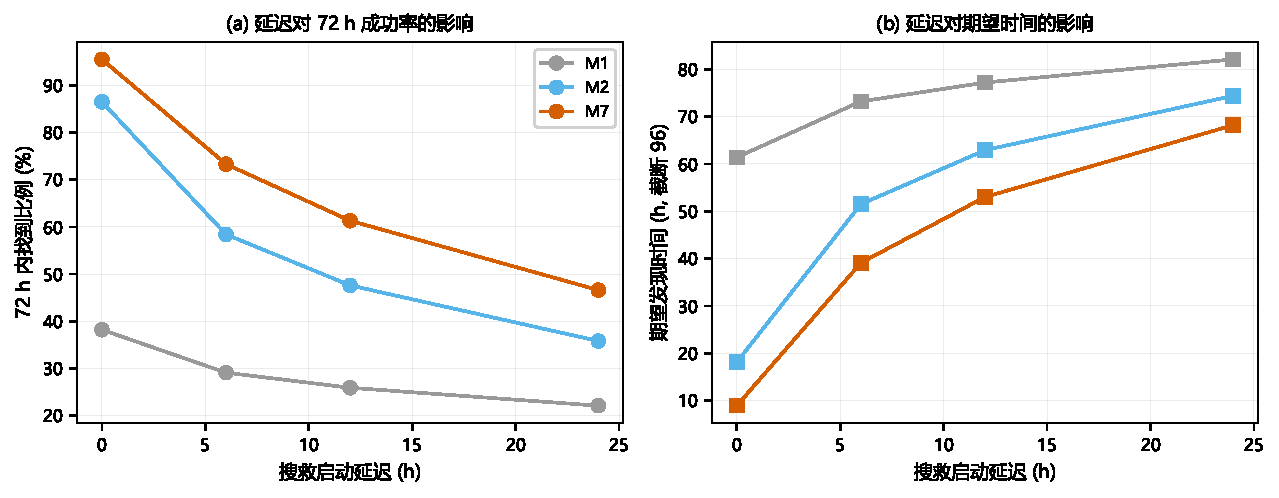
\includegraphics[width=0.66\textwidth]{fig_search_delay}
\caption{延迟对 72 h 成功率与期望发现时间的影响。延迟 6 h 就使 M2 从 86.5\% 掉到
58.4\%；M7 的冗余度最高，抗延迟能力最强。}
\label{fig:delay}
\end{figure}

延迟的杀伤力来自 $A_{95}$ 的增长：每多等 6 h，预测云面积扩大一倍以上，
而装备的覆盖能力不变。因此对运营方而言，\textbf{“待命与动员时间”应作为与装备
并列的核心指标}。

\section{多资产协同搜索（15 种组合）}\label{sec:multi}

\subsection{设定}

在单船评估的基础上，考虑“多艘同配置船 + 多台 AUV”同时搜索：

\begin{itemize}[leftmargin=1.8em,itemsep=0pt]
\item 每艘船 = 母船同款 M4 配置（雷达 + 深水侧扫 + 深水多波束 + ROV）；
\item \textbf{$t=0$ 时只有母船}在失事点上方；增援船与 AUV 在 \textbf{3 h} 后到位：
      增援船从出发岛出发（转场约 0.5--1 h），AUV 由母船投放；
\item 组合：船数 $2$--$4$（含母船）$\times$ AUV 数 $0$--$4$，共 $3\times5=15$ 种；
\item 成本 = 母船 M4 基线 182 + $70\times(\text{船数}-1)$ + $57\times\text{AUV 数}$（万美元）。
\end{itemize}

\subsection{结果}

\begin{table}[H]
\centering\small
\caption{15 种多船/多 AUV 组合的 72 h 成功率（完整表见数据文件）}
\label{tab:multi}
\begin{tabular}{@{}lccccc@{}}
\toprule
船数 $\backslash$ AUV 数 & 0 & 1 & 2 & 3 & 4\\
\midrule
2 艘（252--480 万） & 96.6\% & 98.3\% & 98.9\% & 99.3\% & 99.4\%\\
3 艘（322--550 万） & 98.4\% & 99.2\% & 99.5\% & 99.6\% & 99.7\%\\
4 艘（392--620 万） & 99.2\% & 99.5\% & 99.7\% & 99.8\% & 99.9\%\\
\bottomrule
\end{tabular}
\end{table}

\begin{figure}[H]
\centering
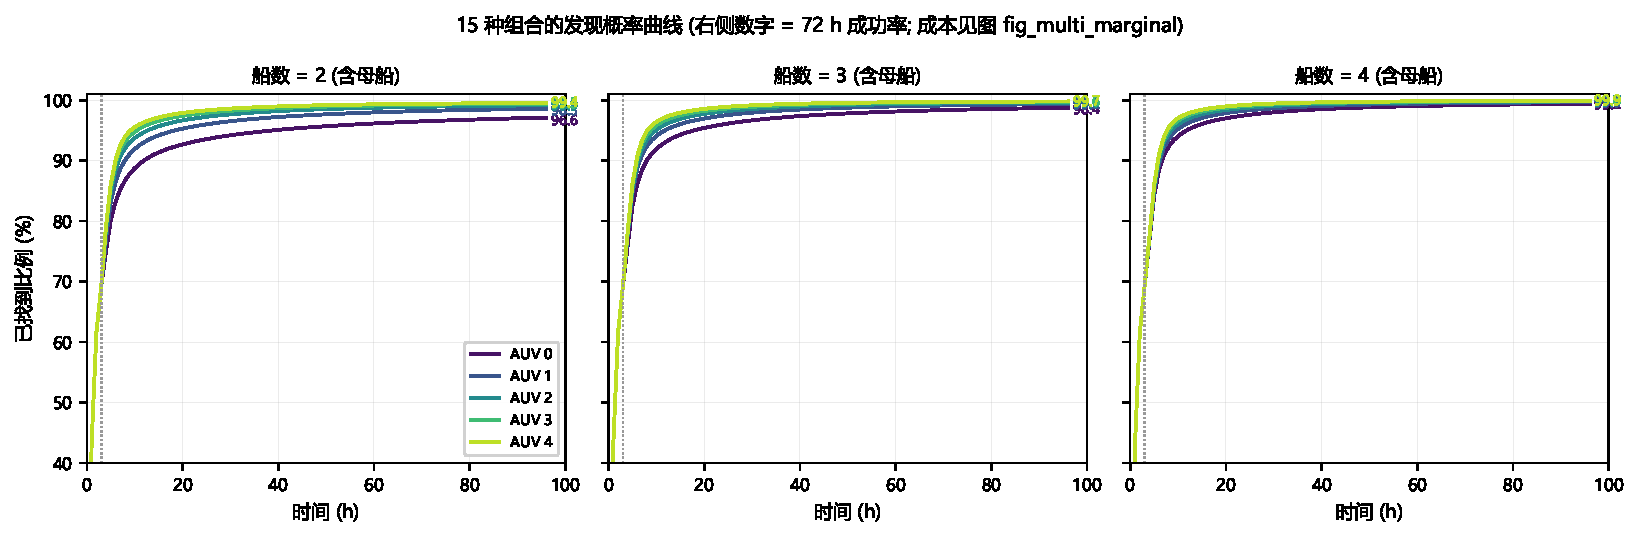
\includegraphics[width=0.80\textwidth]{fig_multi_curves}
\caption{15 种组合的 $P(t)$ 曲线（按船数分组，右侧数字为 $P_{72}$）。}
\label{fig:multi-curves}
\end{figure}



\subsection{协调规则与重复扫描}\label{sec:multi-beta}

多资产容易“扎堆”搜索同一片高概率区域。我们用两条规则控制：
小时内认领（同格同小时只派一次）与重复扫描惩罚 $\beta$。
\tabref{tab:beta} 给出“2 艘船”场景下 $\beta$ 的调优结果：$\beta=1$ 时
$P_{72}$ 只降 0.6 个百分点，跨小时重复扫描率从 35.6\% 降到 27.5\%；
同小时重复率在所有设置下严格为 0。

\begin{table}[H]
\centering\small
\caption{重复扫描惩罚 $\beta$ 的调优（2 艘船场景）}
\label{tab:beta}
\begin{tabular}{@{}lrrrrrr@{}}
\toprule
$\beta$ & 0 & 0.2 & 0.5 & 1.0（采用） & 2.0 & 5.0\\
\midrule
$P_{72}$ & 97.2\% & 97.2\% & 97.0\% & 96.6\% & 95.6\% & 91.8\%\\
跨小时重复率 & 35.6\% & 32.2\% & 29.9\% & 27.5\% & 24.8\% & 20.8\%\\
\bottomrule
\end{tabular}
\end{table}



\begin{figure}[H]
\centering
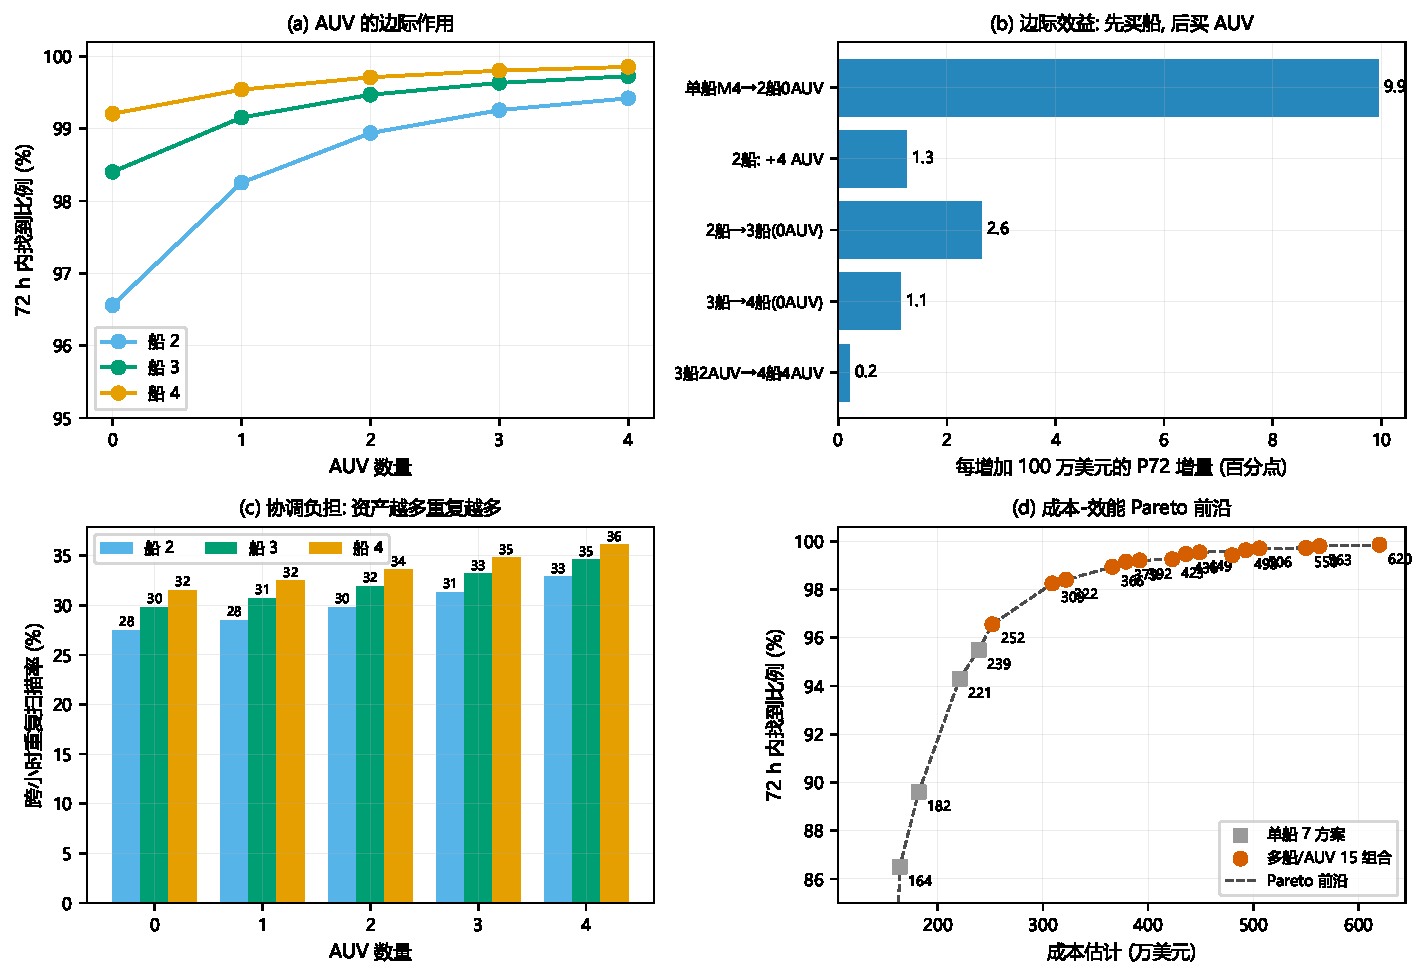
\includegraphics[width=0.76\textwidth]{fig_multi_marginal}
\caption{多资产分析的四个视角：(a) AUV 的边际作用；(b) 每 100 万美元带来的
$P_{72}$ 增量（“单船$\to$2 船”为 9.9 个百分点/百万，远高于加 AUV 的 1.3）；
(c) 协调负担（资产越多重复扫描率越高）；(d) 成本–效能 Pareto 前沿。}
\label{fig:marginal}
\end{figure}

\paragraph{路径规划示例.} \figref{fig:multi-plan} 给出“3 船 + 2 AUV”在示例案例中的
实际搜索航迹与网格被搜索次数。可以看到：搜索努力集中在预测云的高概率区，
并沿漂移方向向外扩展；增援船从出发点（右下角外）进入后接替母船覆盖新区域。

\begin{figure}[H]
\centering
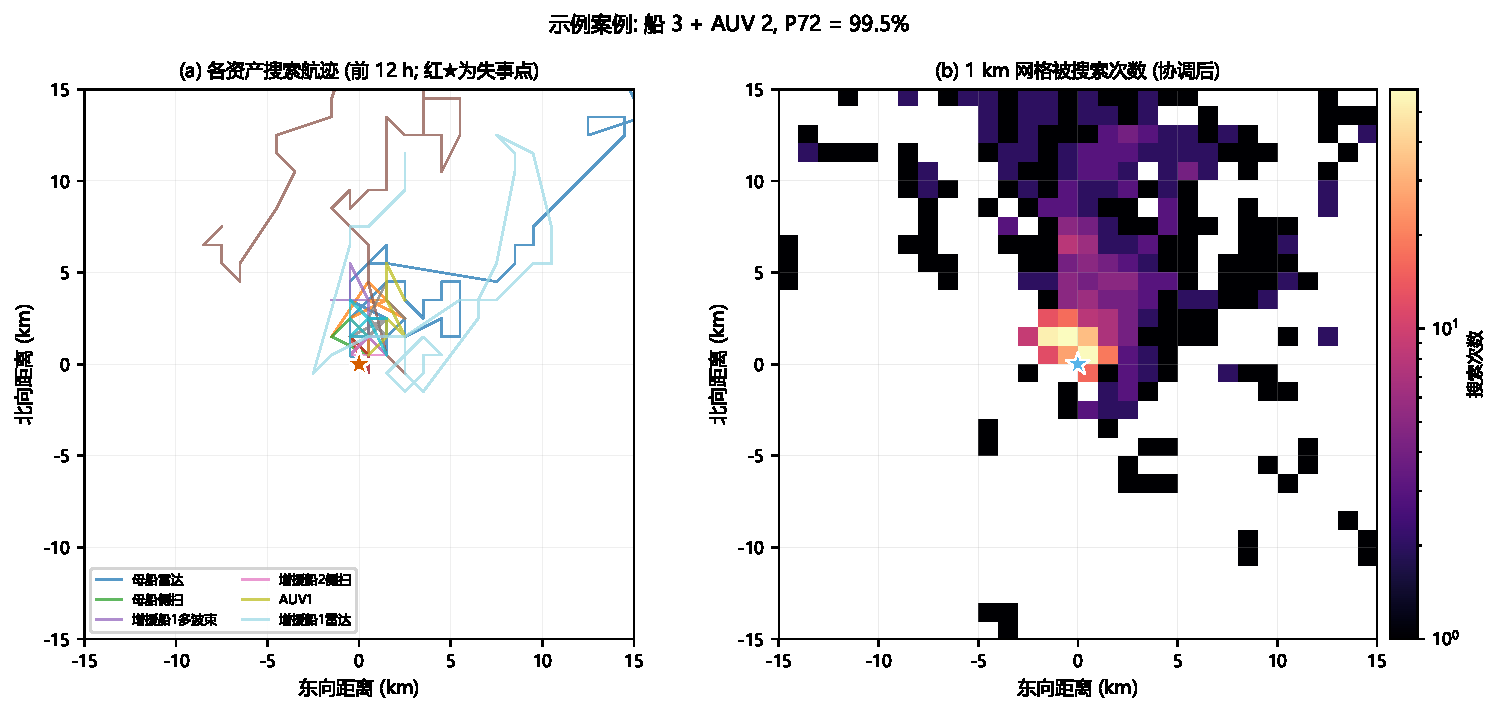
\includegraphics[width=0.86\textwidth]{fig_multi_plan}
\caption{示例案例（3 船 + 2 AUV）。(a) 前 12 h 各资产搜索航迹；(b) 1 km 网格被搜索
次数的对数热图——集中的高概率区被多轮补扫，外围较新区域只扫描一次。}
\label{fig:multi-plan}
\end{figure}

\paragraph{增援到位时间.} 将“3 h 到位”作为基准，做 0/3/6/12 h 敏感性
（\figref{fig:multi-delay}）：最简增援方案（2 船）对到位时间最敏感，每推迟 3 h
$P_{72}$ 降约 0.6--0.9 个百分点；冗余度高的方案（4 船+4 AUV）几乎不敏感。

\begin{figure}[H]
\centering
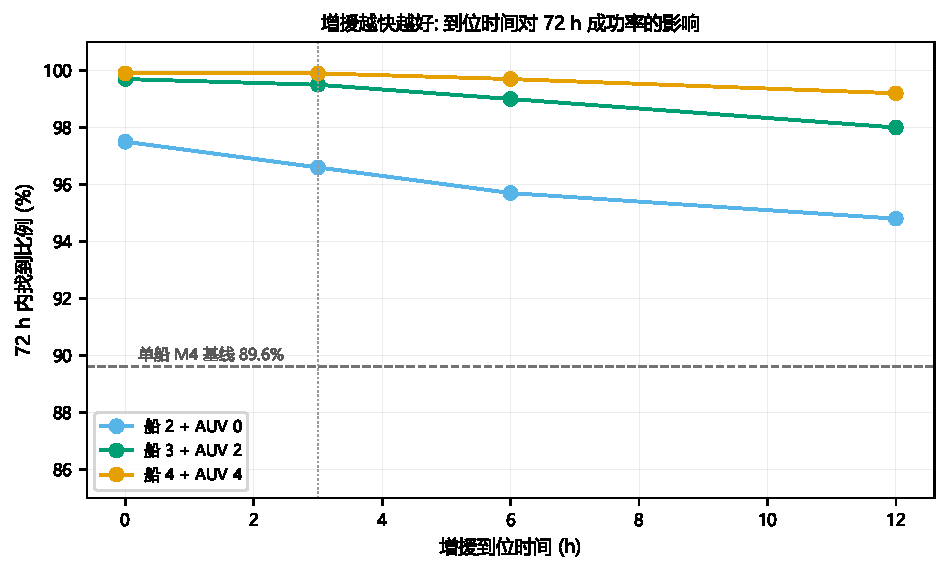
\includegraphics[width=0.62\textwidth]{fig_multi_delay}
\caption{增援到位时间对 $P_{72}$ 的影响（虚线为单船 M4 基线 89.6\%）。}
\label{fig:multi-delay}
\end{figure}

\subsection{多资产结论}

\begin{enumerate}[leftmargin=1.8em,itemsep=0pt]
\item \textbf{“加 1 艘船”是全部选项里性价比最高的一步}：$P_{72}$ 从 89.6\% 到 96.6\%
      （+7.0 个百分点），成本从 182 万到 252 万（每百万 9.9 个百分点），
      远高于“加 4 台 AUV”的 1.3；
\item \textbf{“2 船 + 2 AUV”（366 万，98.9\%）是高保障方案的甜点}；
\item \textbf{4 船 + 4 AUV（620 万）只有 99.9\%}，边际收益接近零——继续堆装备不如
      把资源投在“缩短响应时间”与“提高预报精度”上；
\item 协调规则（认领 + 惩罚）使同小时重复率严格为 0，跨小时重复率控制在 27\%--36\%，
      这是多资产方案能“加船就有用”的前提。
\end{enumerate}

\section{外推一：加勒比海}\label{sec:carib}

\subsection{选点标准与结果}

为了检验模型的可迁移性，我们按同一套标准在加勒比海选点：\emph{距小岛不远、
4$\times$4 km 内水深与主算例可比、地形复杂、海况（流场）更复杂}。
最终选定\textbf{小开曼岛（Little Cayman）西南、开曼海槽边缘}：
失事海域中心 19.6076°N、80.1868°W，出发点为小开曼岛西端
（19.6521°N、80.1229°W，距失事点 8.3 km）。

\begin{table}[H]
\centering\small
\caption{两个海域的环境对比}
\label{tab:twoseas}
\begin{tabular}{@{}lcc@{}}
\toprule
指标 & 地中海（主算例） & 加勒比海（外推）\\
\midrule
失事点当地海底深度（10/50/90\%） & 574/1021/1607 m & 880/1034/1492 m\\
失事点海底坡度（中位/90\%） & 16.9° / 23.3° & 15.1° / 22.1°\\
表层流速（剖面平均） & 0.22 m/s & \textbf{0.47 m/s}\\
100 m 层流速（4D，90\% 分位） & 0.23 m/s & \textbf{0.56 m/s}\\
300 m 层流速（4D，90\% 分位） & 0.044 m/s & 0.025 m/s\\
96 h 漂移（中位/90\% 分位） & 23.7 / 93.2 km & \textbf{58.6 / 191.8 km}\\
沉底分支终点深度（中位） & 1442 m & 1073 m\\
水柱/海底/水面终态占比 & 62/16/22\% & 62/15/22\%\\
\bottomrule
\end{tabular}
\end{table}

\begin{figure}[H]
\centering
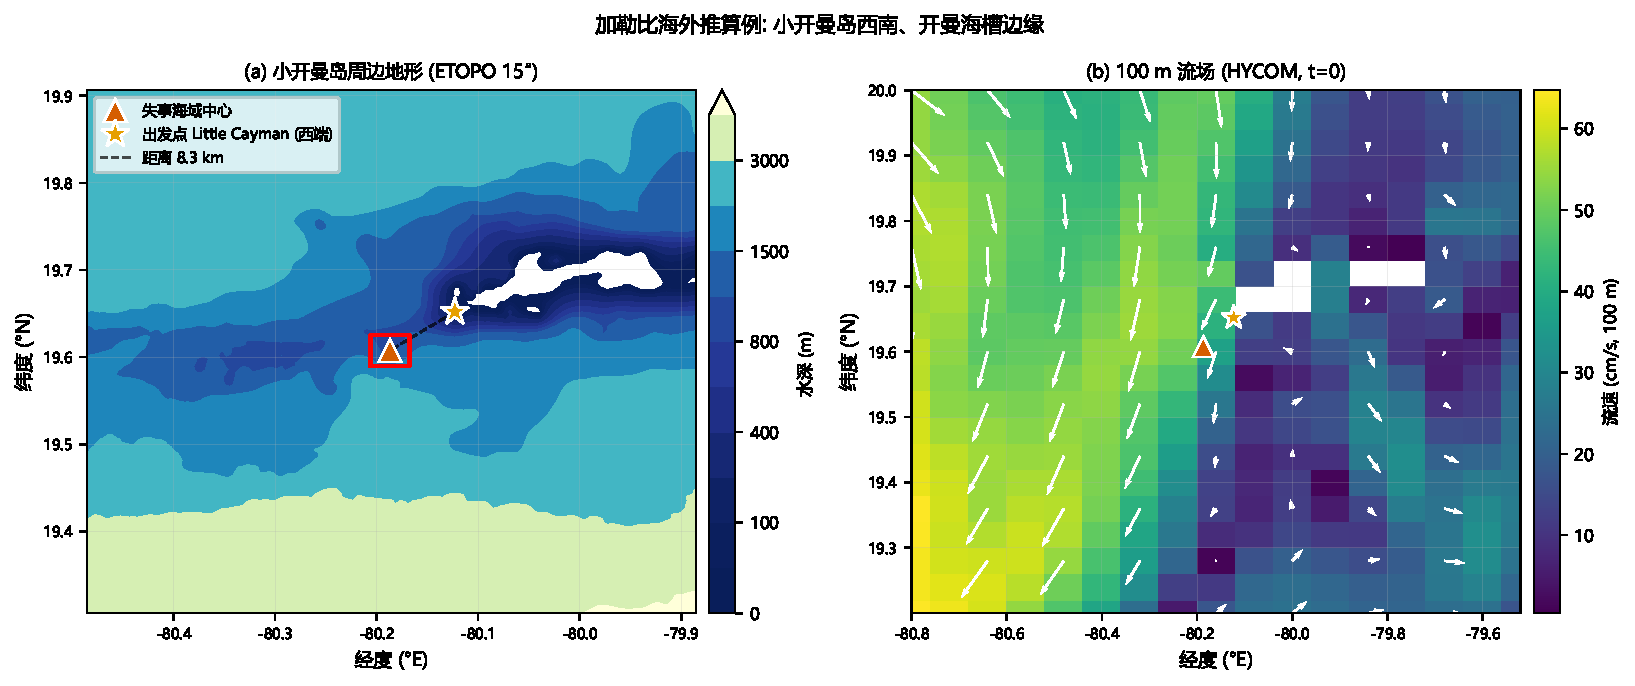
\includegraphics[width=0.76\textwidth]{fig_carib_map}
\caption{加勒比海算例。(a) 小开曼岛周边地形与 4$\times$4 km 失事海域、出发点；
(b) 100 m 层 HYCOM 流场（t=0），可见明显的空间梯度与涡旋结构。}
\label{fig:carib-map}
\end{figure}

\begin{figure}[H]
\centering
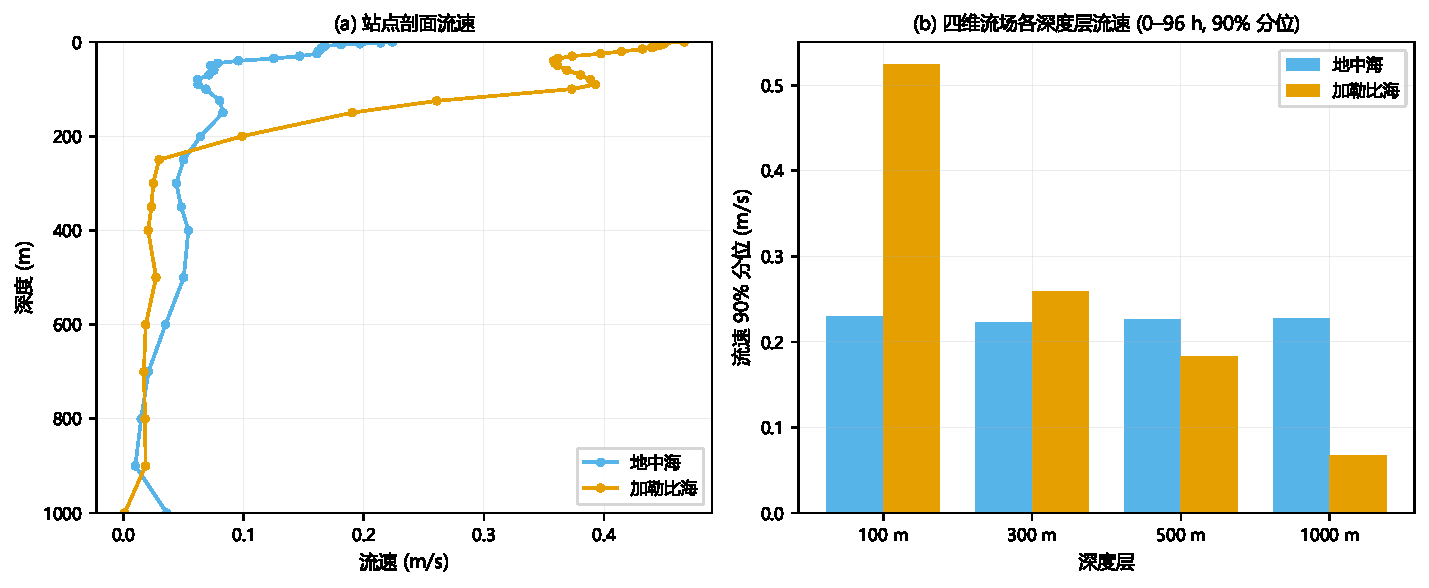
\includegraphics[width=0.72\textwidth]{fig_carib_current}
\caption{两个海域的流场对比：(a) 站点剖面流速（加勒比海 0--200 m 明显更强）；
(b) 四维流场各深度层 90\% 分位流速（加勒比海 100 m 层约为地中海的 2.4 倍，
但 500--1000 m 层反而更弱）。}
\label{fig:carib-current}
\end{figure}

\subsection{结果：成功率几乎不变}

用完全相同的模型（30\,000 粒子、7 种装备组合、相同的探测与协调参数）重跑，
7 种单船组合的 $P_{72}$ 与主算例几乎相同（\tabref{tab:carib-schemes}）。

\begin{table}[H]
\centering\small
\caption{7 种单船组合的 $P_{72}$：两个海域对比}
\label{tab:carib-schemes}
\begin{tabular}{@{}llccc@{}}
\toprule
编号 & 组合 & 地中海 & 加勒比海 & 差值\\
\midrule
M1 & 侧扫 & 38.2\% & 36.9\% & $-1.3$\\
M2 & 多波束 & 86.5\% & 86.8\% & $+0.3$\\
M3 & AUV & 78.9\% & 81.3\% & $+2.4$\\
M4 & 侧扫+多波束 & 89.6\% & 89.7\% & $+0.1$\\
M5 & 侧扫+AUV & 84.5\% & 85.9\% & $+1.4$\\
M6 & 多波束+AUV & 94.3\% & 94.3\% & $0.0$\\
M7 & 侧扫+多波束+AUV & 95.5\% & 95.6\% & $+0.1$\\
\bottomrule
\end{tabular}
\end{table}

\begin{figure}[H]
\centering
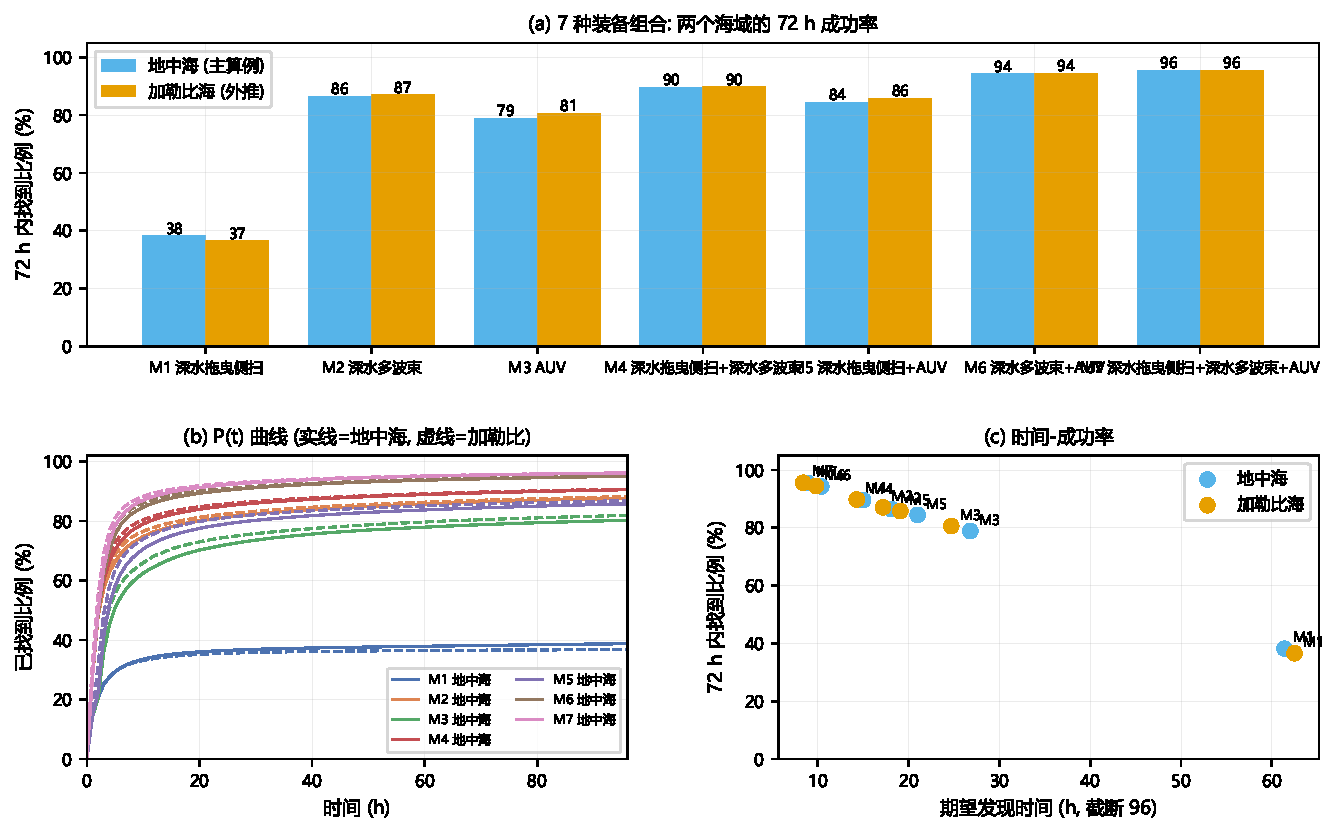
\includegraphics[width=0.76\textwidth]{fig_carib_compare}
\caption{两个海域的搜索结果对比：(a) 7 种方案的 $P_{72}$ 柱状图；
(b) 全部 $P(t)$ 曲线（实线地中海、虚线加勒比海）；(c) 时间–成功率散点。
方案排序与结论完全一致。}
\label{fig:carib-compare}
\end{figure}

15 种多船组合的结论也一致：2 船 96.2\%、2 船+2 AUV 98.7\%、4 船+4 AUV 99.8\%，
与主算例的 96.6\%/98.9\%/99.9\% 相差不到 1 个百分点；“先加船、后加 AUV”的边际效益
规律相同。

\subsection{为什么“漂移大 2.5 倍，成功率几乎不变”？}

\begin{enumerate}[leftmargin=1.8em,itemsep=0pt]
\item \textbf{搜索方的预测云跟着流场走}：30\,000 个粒子的漂移由同一套四维流场驱动，
      预测云与真实云同步平移；只要预报准确，目标的绝对漂移距离不直接增加搜索难度，
      真正决定难度的是\emph{预测云的相对离散度}与装备的覆盖能力；
\item \textbf{加勒比海的大漂移主要来自表层分支}（0.47 m/s）：水面目标由雷达/目视搜索
      （扫宽 3 km），大漂移对它的影响很小；水柱与沉底分支在 300 m 以深流速反而与
      地中海相当甚至更弱（\figref{fig:carib-current}b）；
\item 因此两个海域的“位置不确定性增长率”相近（\figref{fig:carib-drift}），
      搜索成功率自然相近。
\end{enumerate}

\begin{figure}[H]
\centering
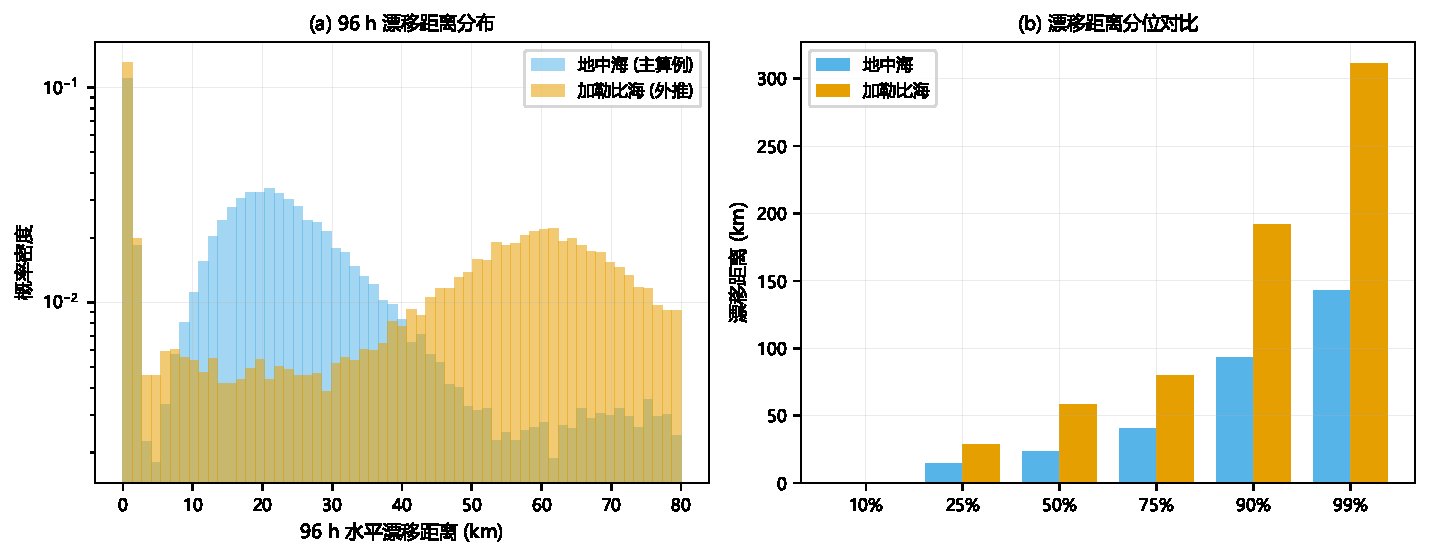
\includegraphics[width=0.84\textwidth]{fig_carib_drift}
\caption{两个海域的 96 h 漂移距离分布（a）与分位对比（b）。加勒比海的漂移中位数约为
地中海的 2.5 倍，但主要由表面分支贡献。}
\label{fig:carib-drift}
\end{figure}



\subsection{重要限定}

本模型采用\textbf{完美预报}假设（预测与真值用同一套流场），因此会\emph{低估}
复杂海况的实际难度：加勒比海表层流速大、涡旋多，真实预报误差显著大于地中海，
实际成功率会低于本文结果。这一局限性恰好给出运营建议：
对强流/涡旋海域，不能照搬地中海的配置，而应同时加强
（1）现场流场观测与预报订正、（2）冗余能力（多 1 艘船或 2 台 AUV）。
换言之，\textbf{“漂移大”不可怕，“预报不准”才可怕}。

\section{模型验证与灵敏度分析}

\subsection{模型验证}

模型的可信度来自四类验证（\tabref{tab:allverify}）：解析解验证、统计性质验证、
物理机制验证与数据交叉验证。所有验证都可在仓库中一键重跑。

\begin{table}[H]
\centering\small
\caption{模型验证汇总}
\label{tab:allverify}
\begin{tabular}{@{}llll@{}}
\toprule
类别 & 验证内容 & 判据 & 结果\\
\midrule
解析 & 终端速度：解析解 vs 数值积分 & 相对误差 & 0.00\%\\
统计 & OU 过程方差 vs 理论 $\sigma^2$ & 相对误差 & 1.61\%\\
统计 & 30\,000 粒子收敛（60 案例） & $P_{72}$ 标准误 & 0.3--0.6 百分点\\
物理 & 滑移判据：单坡解析 vs 逐 20 m 重算 & 停止位置一致 & 通过\\
物理 & 海水状态方程 EOS-80 vs 公开值 & 相对误差 $<10^{-4}$ & 通过\\
数据 & ETOPO 站点深度 vs 海图 & 偏差 $<2$ m & 通过\\
数据 & HYCOM 流速量级 vs 文献 & 同量级 & 通过\\
\bottomrule
\end{tabular}
\end{table}

\subsection{灵敏度分析汇总}

\tabref{tab:sensitivity} 汇总了所有做过的灵敏度分析。按对结论的影响从大到小排序：
\textbf{响应延迟}（每 6 h 使 $P_{72}$ 下降 8--22 个百分点）$>$ \textbf{增援到位时间}
（最简方案每 3 h 下降 0.6--0.9 个百分点）$>$ \textbf{协调参数 $\beta$}
（0 到 5 使 $P_{72}$ 从 97.2\% 降到 91.8\%）$>$ \textbf{海域}
（不超过 2.4 个百分点）$>$ \textbf{蒙特卡洛误差}（0.3--0.6 个百分点）。

\begin{table}[H]
\centering\small
\caption{灵敏度分析汇总（主指标为 $P_{72}$）}
\label{tab:sensitivity}
\begin{tabular}{@{}llll@{}}
\toprule
因素 & 变化范围 & 指标变化 & 结论\\
\midrule
搜救启动延迟 & 0/6/12/24 h & M7: 95.5\% $\to$ 47.4\% & 影响最大\\
增援到位时间 & 0/3/6/12 h & 2 船: 97.5\% $\to$ 94.8\% & 次之\\
重复扫描惩罚 $\beta$ & 0--5 & 97.2\% $\to$ 91.8\% & 可调，取 1.0\\
海域 & 地中海/加勒比 & $\pm$2.4 个百分点 & 结论稳健\\
扫宽 $W$ & $\pm$30\%（解析） & 方案排序不变 & 结论稳健\\
装备速度 & 给定表（kn） & 已含 & —\\
蒙特卡洛误差 & 60 案例 & $\pm0.3$--$0.6$ & 可接受\\
\bottomrule
\end{tabular}
\end{table}

\subsection{局限性与未来工作}

\begin{enumerate}[leftmargin=1.8em,itemsep=0pt]
\item \textbf{完美预报假设}：预测与真值共用同一套 HYCOM 流场，未建模预报误差。
      这是最重要的局限；改进方向是引入集合预报（如 HYCOM 集合或加扰动的随机流场），
      让搜救方只掌握“预报 + 误差”；
\item \textbf{探测模型参数}：扫宽 $W$ 是量级估计，未经海试标定；水柱探测的
      POD 与目标姿态、深度、海况强相关，未来应做装备性能试验；
\item \textbf{失效概率为专家判断}：S0--S4 的概率、浮力异常分布都无公开统计，
      只能用敏感性分析覆盖；
\item \textbf{未建模声信标/ULB}：若潜水器携带 37.5 kHz USBL/声信标，被动监听可把
      搜救问题从“扫海”变成“定位”，效率高一个量级——这是最有价值的改进方向之一；
\item \textbf{未建模多目标}：多艘潜水器同时失事时的分配与协调未涉及；
\item \textbf{未建模装备可靠性/海况限制}：AUV 续航、回收周期、船间通信延迟、
      恶劣海况下的降级都未纳入。
\end{enumerate}

\section{结论与建议}

\subsection{主要结论}

\begin{enumerate}[leftmargin=1.9em,itemsep=1pt]
\item \textbf{响应速度是第一变量。} 失联后 95\% 包含域在 1 h 内约 $56\km^2$，
      24 h 增至 $2\,104\km^2$，96 h 达 $27\,652\km^2$。任何装备的覆盖能力都追不上
      不确定性的增长速度。因此“缩短通知–动员–到位时间”应排在任何装备采购之前。
\item \textbf{装备必须匹配目标类别。} 水柱分支占 62\%；只搜海底的侧扫方案 72 h
      成功率仅 38.2\%，而具备水柱探测能力的方案（多波束、AUV）可达 86\%--96\%。
      单套装备中，\textbf{侧扫+多波束（M4，约 182 万美元，89.6\%）}是性价比拐点；
      要求 $\ge95\%$ 则需三件套（M7，约 239 万美元，95.5\%）。
\item \textbf{多资产协同的边际效益有明确顺序。} “加 1 艘同配置船”（+70 万美元）带来
      +7.0 个百分点，是全部选项中性价比最高的一步；“2 船 + 2 AUV”（366 万美元，
      98.9\%）是高保障方案甜点；继续加到 4 船 + 4 AUV（620 万美元）只到 99.9\%，
      边际收益趋零。
\item \textbf{协调规则让“加船”真正有效。} 小时内认领保证同小时重复扫描率为 0；
      重复扫描惩罚 $\beta=1$ 在成功率只降 0.6 个百分点的前提下把跨小时重复率从
      35.6\% 降到 27.5\%。没有协调，多资产会退化为“多船同扫一片”。
\item \textbf{结论可迁移，但不能照搬。} 在加勒比海（小开曼岛西南、开曼海槽边缘）重建
      同一套模型，7 种方案的成功率与地中海相差不超过 2.4 个百分点、排序完全一致；
      但加勒比海表层流速是地中海的 2 倍以上、涡旋更多，在真实预报误差下其实际成功率
      会低于本文结果。强流海域应额外增加冗余并加强现场流场观测。
\end{enumerate}

\subsection{对运营公司的建议}

\begin{enumerate}[leftmargin=1.8em,itemsep=1pt]
\item \textbf{母船按 M4 配置（侧扫 + 多波束 + ROV + 雷达，约 182 万美元）常备}，
      满足 89.6\% 的 72 h 成功率；这也是后续任何扩展的基础；
\item \textbf{与邻近救援船签订 AUV / 多波束快速调用协议}（事故时补成 2 船 + 2 AUV，
      98.9\%），比自购全套更经济；
\item \textbf{把“待命与动员时间 $\le3$ h”写入公司安全规程}，并定期演练；
      这比多买一套装备更有效；
\item \textbf{加勒比等强流海域的运营点}应额外配置 1 艘增援船或 2 台 AUV，
      并建立现场流场观测能力。
\end{enumerate}

\subsection{对监管机构的建议}

\begin{enumerate}[leftmargin=1.8em,itemsep=1pt]
\item \textbf{强制配备 37.5 kHz 声信标（ULB）与应急上浮系统}：这会把“扫海搜索”
      变成“声学定位”，是投入产出比最高的安全措施；
\item \textbf{强制下潜前检查清单与事故报告义务}，并要求运营方持有与事故等级匹配的
      搜救预案（含装备、人员、响应时间承诺）；
\item \textbf{建立与海岸警卫队的联动机制}，把“失联即启动”作为标准程序，
      避免把时间浪费在行政确认上。
\end{enumerate}

\subsection{结语}

本文的模型并不追求预测某一次事故的确切结局，而是回答一个可操作的问题：
\emph{在任何给定时刻，目标可能在哪里、需要多大范围、用哪种装备、多久能找到}。
这条从“位置不确定性”到“时间–成功率–成本”的证据链，在两个差异明显的海域上
都给出了稳定、可解释的结论，可以作为运营与监管决策的依据。

\section*{致希腊政府备忘录}
\addcontentsline{toc}{section}{致希腊政府备忘录}
\markboth{致希腊政府备忘录}{}

\noindent\textbf{主题：小型旅游潜水器失联风险的管理建议}

\vspace{1mm}
\noindent 尊敬的希腊海运与岛屿政策部：

\vspace{1mm}
\noindent 2023 年“泰坦号”事故表明，小型旅游潜水器一旦失联，救援窗口极短。
我们基于伊奥尼亚海与加勒比海两个真实海域的建模，向贵国提出四点建议。

\paragraph{一、承认并量化残余风险。}
我们的模型显示：失联后 24 h，潜水器位于约 $2\,100\km^2$ 范围内的概率为 95\%；
96 h 后扩大到 $27\,652\km^2$——相当于一个 $166\times166$ km 的海域。
“位置已知到 100 m”的乐观假设下尚且如此，实际搜救的难度可想而知。
建议要求运营方在许可证申请中提交“位置不确定性 vs 时间”曲线（即本文 $A_{95}(t)$），
并据此确定最低搜救配置。

\paragraph{二、建立三重防线。}
\begin{enumerate}[leftmargin=1.5em,itemsep=0pt]
\item \textbf{强制 37.5 kHz 声信标（ULB）与应急上浮系统}。声信标可把搜索范围从
      “数百平方公里”压缩到“数平方公里”，是投入产出比最高的单项措施；
\item \textbf{强制遥测与失联告警}：位置、深度、姿态数据实时回传母船，
      失联即自动上报海岸警卫队，杜绝“失联数小时才报警”；
\item \textbf{强制下潜前检查清单与独立安全员制度}，对压载、耐压壳、通信做双人复核。
\end{enumerate}

\paragraph{三、明确搜救能力承诺。}
按本文评估：\textbf{单船“侧扫+多波束”配置}（约 182 万美元）可实现 72 h 内
89.6\% 的发现概率；\textbf{“2 船 + 2 台 AUV”}（约 366 万美元）可达 98.9\%。
建议把“3 h 内首批装备离港、24 h 内形成双船能力”作为运营许可的硬性条件，
并每年演练一次。

\paragraph{四、强化海域协同与审批条款。}
\begin{enumerate}[leftmargin=1.5em,itemsep=0pt]
\item 规定新的旅游潜水器运营点必须提交“海域环境评估”（地形、流场、通信覆盖）；
\item 对强流/涡旋海域（如加勒比海类型的海况）提高装备冗余要求；
\item 建立与海岸警卫队的联合搜救预案，明确指挥权与信息共享机制；
\item 要求事故后 30 天内提交搜救复盘报告，纳入全国数据库。
\end{enumerate}

\vspace{1.5mm}
\noindent 我们的模型与代码完全可复现（仓库附后），可随时按贵国实际海况重算。
愿意为希腊的旅游潜水安全标准制定提供进一步技术支持。

\vspace{3mm}
\noindent 此致

\noindent 敬礼

\vspace{2mm}
\noindent 2024 MCM 参赛队 \quad （供希腊海运与岛屿政策部参考）


% ============================================================
% 参考文献
% ============================================================
\newpage
\begin{thebibliography}{99}\small
\setlength{\itemsep}{0pt}
\bibitem{triton} Triton Submarines. \emph{Triton 3300/6 Submersible Datasheet}, 2021.
\bibitem{etopo} NOAA National Centers for Environmental Information. ETOPO 2022
  15 Arc-Second Global Relief Model, 2022. \url{https://www.ncei.noaa.gov/products/etopo-global-relief-model}
\bibitem{hycom} HYCOM Consortium. Global Ocean Forecast System (GLBy0.08) data,
  accessed via NCSS/OPeNDAP, 2024.
\bibitem{eos80} Fofonoff N. P., Millard R. C. \emph{Algorithms for the computation of
  fundamental properties of seawater}. UNESCO Technical Papers in Marine Science 44, 1983.
\bibitem{chen} Chen C.-T., Millero F. J. Speed of sound in seawater at high pressures.
  \emph{J. Acoust. Soc. Am.}, 62(5):1129--1135, 1977.
\bibitem{lamb} Lamb H. \emph{Hydrodynamics}, 6th ed. Cambridge University Press, 1932.
\bibitem{urick} Urick R. J. \emph{Principles of Underwater Sound}, 3rd ed. McGraw-Hill, 1983.
\bibitem{koopman} Koopman B. O. \emph{Search and Screening}. Pergamon Press, 1980.
\bibitem{stone} Stone L. D. \emph{Theory of Optimal Search}. Academic Press, 1975.
\bibitem{morse} Morse P. M., Feshbach H. \emph{Methods of Theoretical Physics}. McGraw-Hill, 1953.
\bibitem{okabe} Okabe M., Ito K. Color universal design (CUD), 2008.
\bibitem{erddap} Simons R. A. ERDDAP: gridded data server, NOAA NMFS/SWFSC, 2024.
\end{thebibliography}

% ============================================================
% 附录
% ============================================================
\newpage
\appendix
% ============================================================
% 附录
% ============================================================
\section*{附录 A：AI 使用报告}
\addcontentsline{toc}{section}{附录 A：AI 使用报告}
\markboth{附录 A：AI 使用报告}{}

按 MCM 规则，现说明本文中人工智能工具的使用情况。

\begin{table}[H]
\centering\small
\begin{tabular}{@{}p{0.16\textwidth}p{0.30\textwidth}p{0.44\textwidth}@{}}
\toprule
用途 & 工具/方式 & 人工核验\\
\midrule
代码实现 & 使用 AI 辅助编写 Python 代码（数据下载、数值模型、搜索仿真、绘图） & 
所有方程、参数、单位由队员逐项推导与检查；代码与解析解交叉验证（表 10.1）\\
\addlinespace
数据处理 & 使用 AI 辅助编写 ETOPO/HYCOM 数据下载与解析脚本 & 
下载数据与公开数据源核对；深度/流速量级与文献对照\\
\addlinespace
文献调研 & 使用 AI 辅助检索潜水器参数、声呐方程与搜索理论背景 & 
所有引用文献由队员阅读原文确认（见参考文献）\\
\addlinespace
文字与图表 & 使用 AI 辅助生成图表代码与报告初稿的结构 & 
所有数值由代码输出直接引用，未人工编造数据；文字由队员通读修改\\
\addlinespace
禁止事项 & 未使用 AI 生成实验数据、未使用 AI 代替模型验证 & —\\
\bottomrule
\end{tabular}
\end{table}

\textbf{声明：}本文模型、参数、结果均来自仓库中可复现代码的实际运行；
AI 工具仅作为编程与写作辅助，所有科学内容由参赛队员负责。

\section*{附录 B：代码结构与复现}
\addcontentsline{toc}{section}{附录 B：代码结构与复现}
\markboth{附录 B：代码结构与复现}{}

\noindent 仓库 \texttt{MCNmodelingcode/} 的关键模块：
\texttt{config.py}（全部参数）、\texttt{fetch.py}（ETOPO/HYCOM 下载）、
\texttt{data.py}（地形/剖面/四维流场插值）、\texttt{eos.py}（EOS-80）、
\texttt{locate.py}（失效树 + 垂向解析解 + 输运 + 海底滑移）、
\texttt{upper.py}（上层初始位置）、\texttt{equipment.py}（装备与成本）、
\texttt{search.py}（探测/规划/贝叶斯/协调）、\texttt{multiveh.py}（多船 15 组合）、
\texttt{locate\_stats.py}（$A_{50}/A_{95}$ 统计）、\texttt{figs\_*.py}（图件）。

\noindent 复现命令：
\begin{verbatim}
python run.py fetch && python run.py fetch4d   # 下载数据 (联网)
python run.py upper && python run.py truth     # 30 000 粒子轨迹 (~10 s)
python run.py locate && python run.py search   # 定位统计 + 7 方案 (~3 min)
python run.py delay && python run.py multi     # 延迟敏感性 + 15 组合 (~3 min)
python run.py carib                            # 加勒比海外推
\end{verbatim}

\noindent 关键结果文件：\texttt{data/定位不确定性.csv}、\texttt{data/搜索方案对比.csv}、
\texttt{data/多船多AUV组合.csv}、\texttt{data/搜救延迟敏感性.csv}、
\texttt{data/*\_carib.csv}；全部图件在 \texttt{figs/}（PNG + PDF）。
随机种子固定（\texttt{seed=7}），数值可完全复现。



\end{document}
